\setRL
\clearpage
\pagenumbering{arabic} 


\section{
مقدمه
}
برای مدل‌سازی غشاها ابتدا پوسته‌های نازک را بررسی خواهیم کرد. توصیف پوسته‌های نازک را با بررسی انرژی خمشی و انرژی کششی یک محیط پیوسته آغاز خواهیم کرد. پس حل معادلات پیوسته، این معادلات را برای مجموعه نقاط در فضا که بر روی شبکه‌ی مثلثی قرار دارند حل می‌کنیم. سپس تغییرات انرژی در صورت ایجاد نقاط نقص بر روی شبکه را محاسبه خواهیم کرد. 


مقاله الکساندرا مرجع ۷ در مقده تيوری خیلی خوب راجع به آنالیز فرکانس نوشته


\begin{figure}[h]
\begin{center}
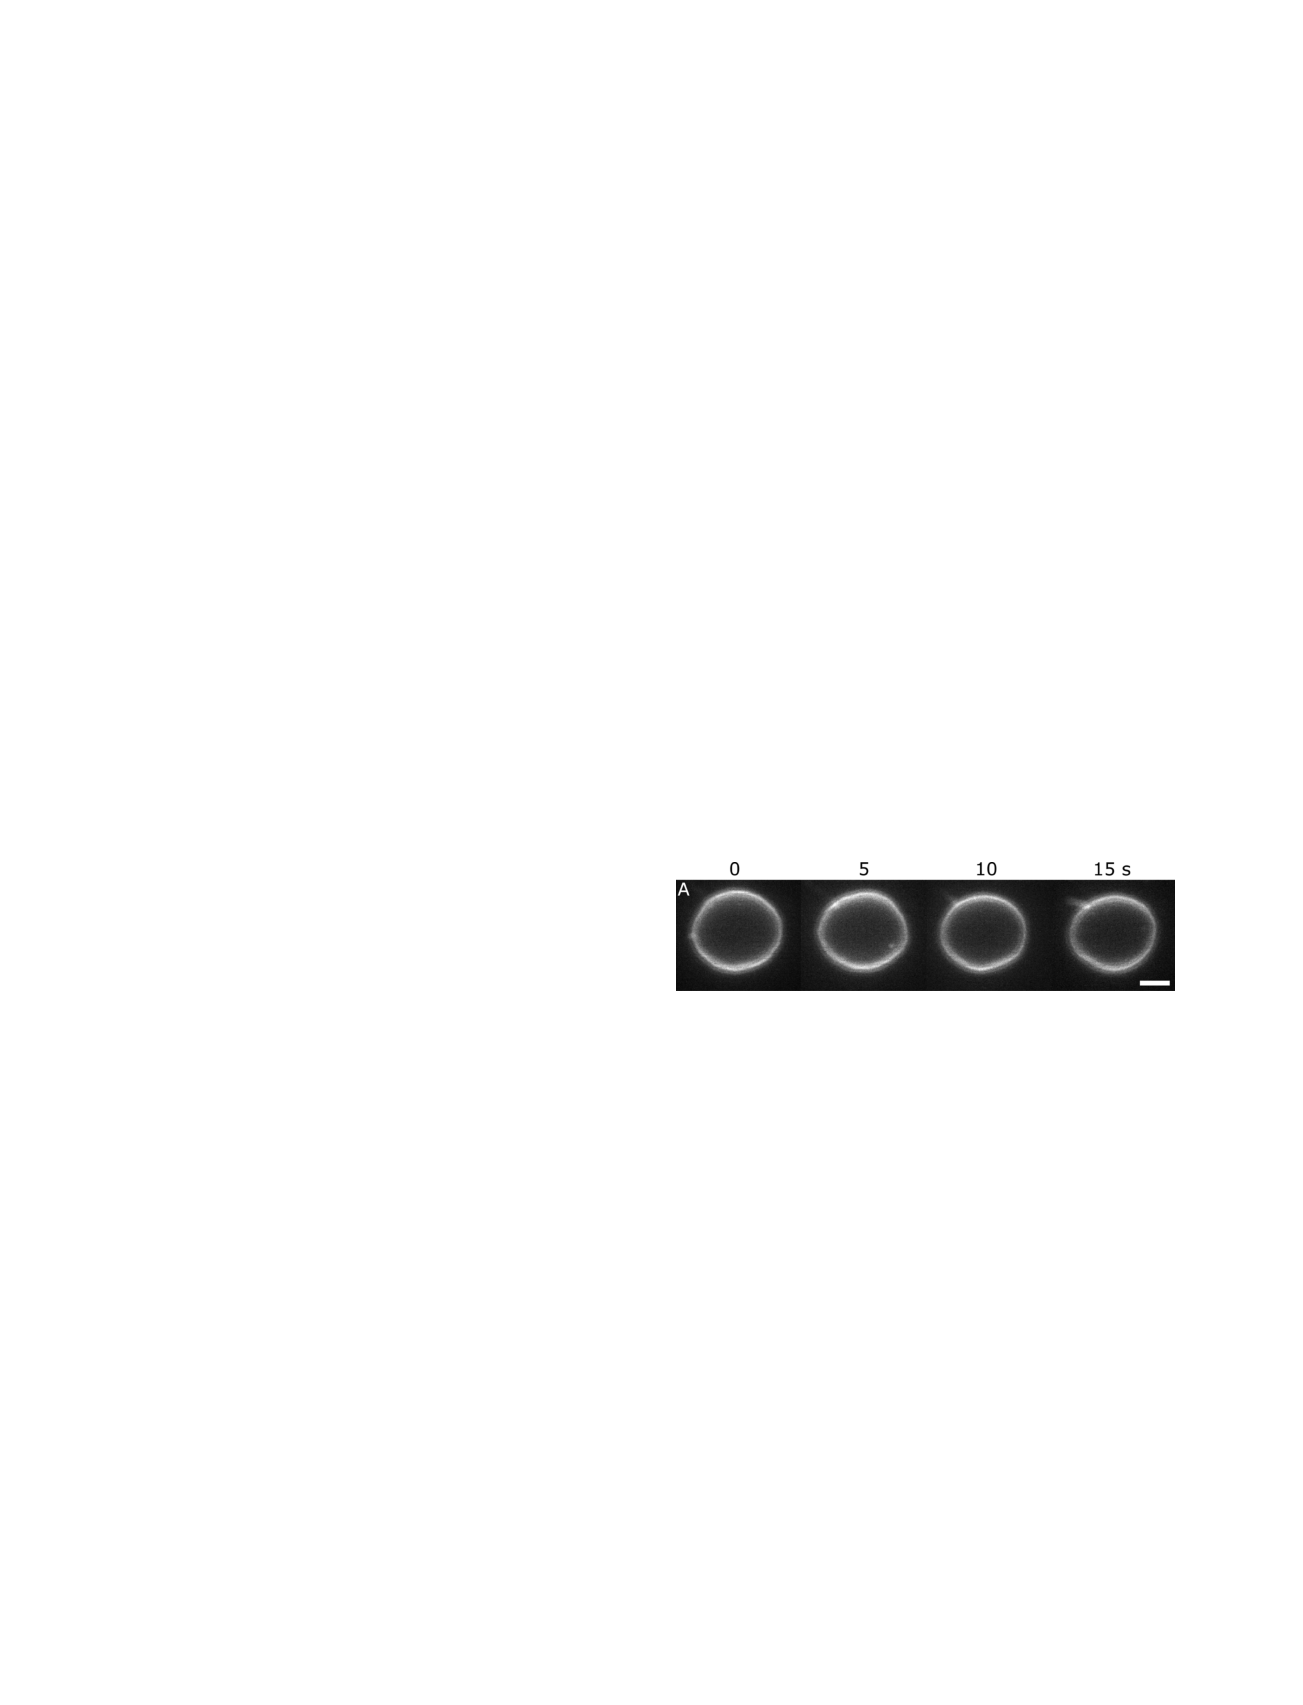
\includegraphics[width=4in]{Membrane_fluctuations}
\caption{
مجموعه تصاویر پست سر هم از تغییر شکل یک غشای لیپیدی را با تصویر برداری فلورسانت در بازه‌های ۵ ثانیه‌ای نشان می‌دهد. خط مقیاس سفید رنگ اندازه‌ی ۵ میکرومتر را نشان می‌دهد. 
\cite{ParthasarathyMembraneMeasurement}
}
\label{fig:flucmem}
\end{center}
\end{figure}

شگل 
\ref{fig:flucmem}
تغییر شکل یک غشای لیپیدی غول آسا (قطر حدود ۱۰ میکرون) در بازه‌های زمانی ۵ ثانیه نشان می‌دهد
\cite{ParthasarathyMembraneMeasurement}
. از نظر انرژی تغییر شکل این غشا را می‌توان به دو بخش کلی تقسیم کرد. تغییر انرژی ناشی از خم شدن و تغییر حاصل از کشش سطح غشا. شکل
\ref{fig:elasticdeformation}
الف، تغییر شکل یک عنصر سطحی بر اثر خمش را نشان می‌دهد. خمش سطح را می‌توان با اندازه‌ی شعاع دو دایره که بر عنصر سطح مماس هست، توصیف کرد. همچنین شکل 
\ref{fig:elasticdeformation}
ب، تغییر شکل عنصر سطح به علت ایجاد کشش در سطح نشان می‌دهد. تغییر سطح با اختلاف مساحت عنصر سطح با حالت کشیده نشده توصیف می‌شود.
\begin{figure}[h]
\begin{center}
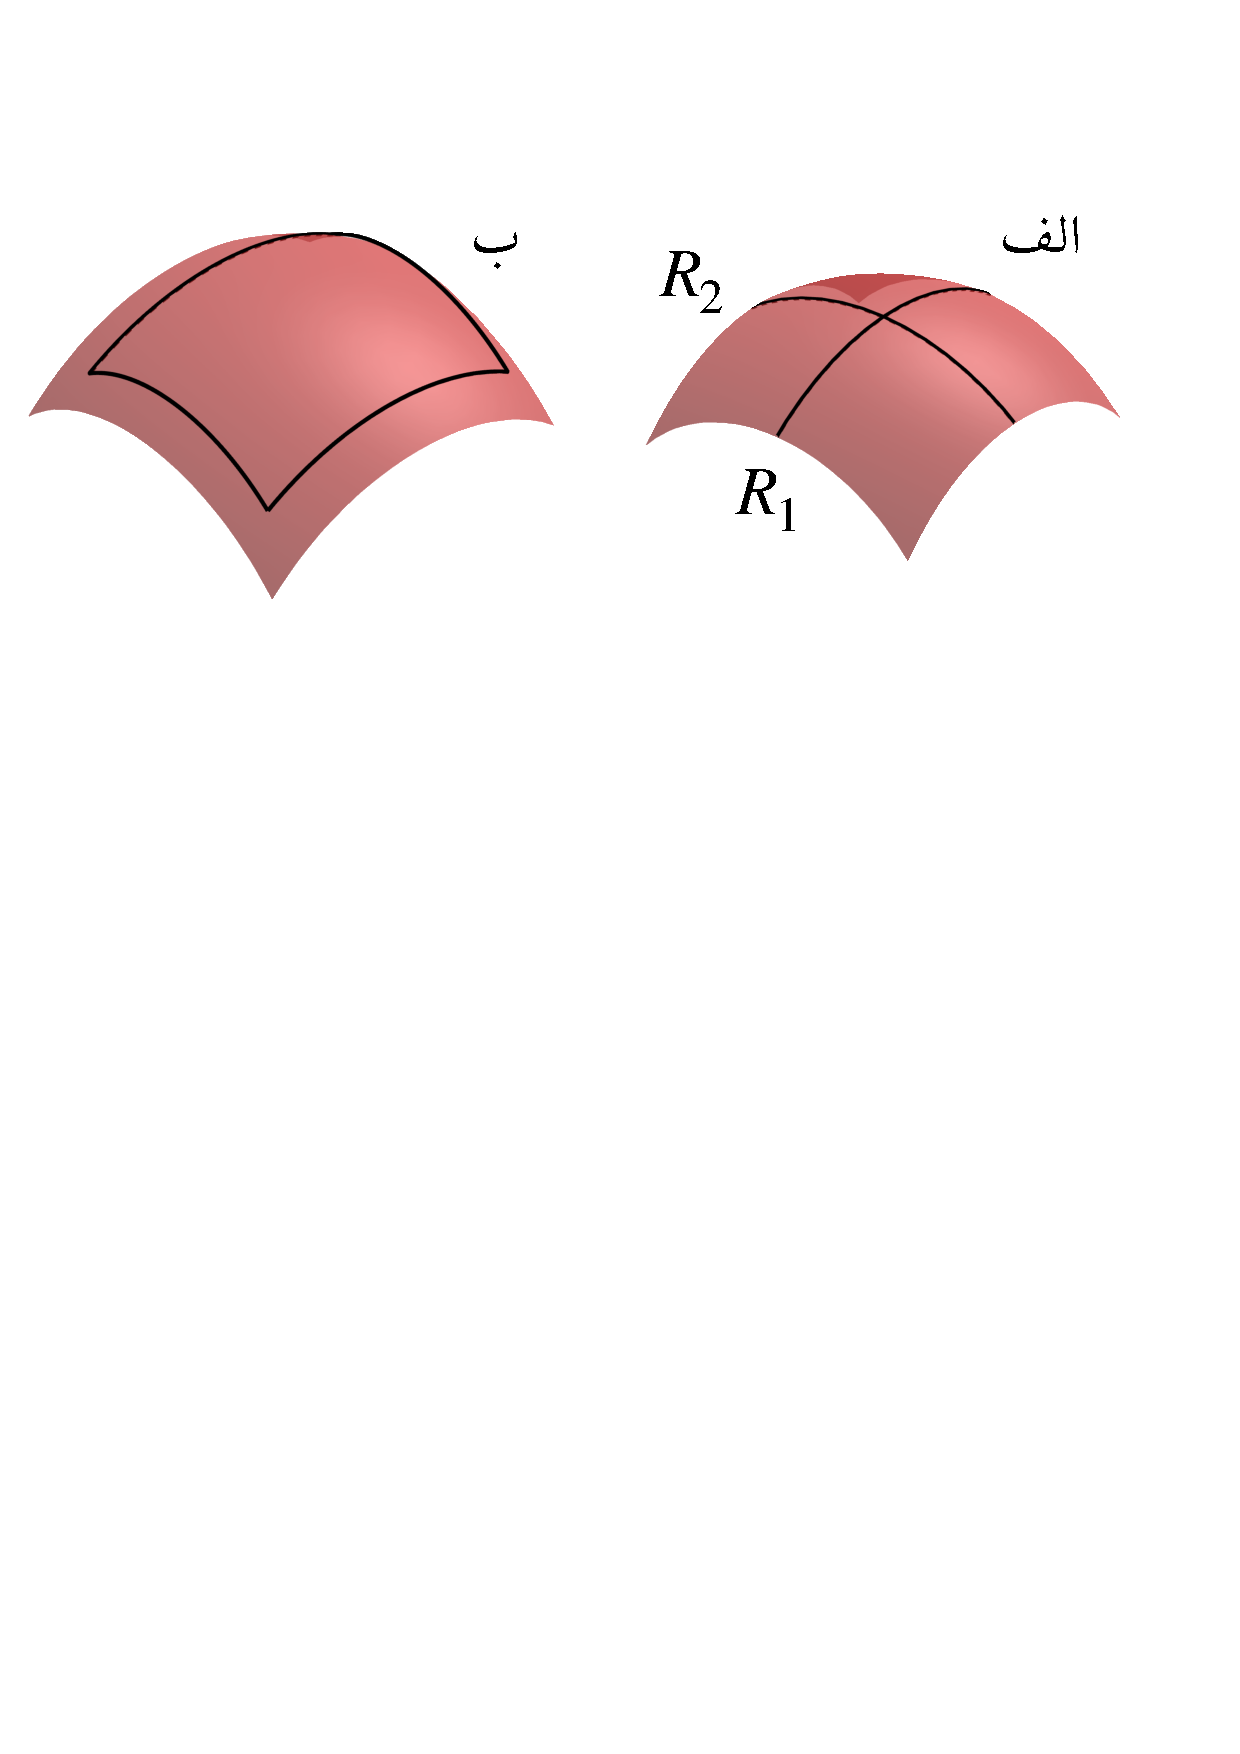
\includegraphics[width=4in]{surface elemnts.pages.pdf}
\caption{
تغییر شکل عنصر سطحی بر اثر الف، خمش و ب، کشش.
}
\label{fig:elasticdeformation}
\end{center}
\end{figure}

\subsection{
انرژی کشش در سطح
}
اگر فرض کنیم جابجایی روی یک عنصر سطحی حاصل از کشیده‌ یا فشرده شدن سطح با بردار 
$u$
توصیف شود، با فرض خطی بودن عکس العمل ماده، انرژی پتانسیل حاصل از تغییر شکل سطح را می‌توان با معادله‌ی زیر بررسی کنیم.

\begin{equation}
E_{stretching}=\frac{1}{2}Y_{2D}A\varepsilon^2
\end{equation}
که اینجا 
$Y_2D$
مدول دو بعدی یانگ،
$A$
سطح عنصر در حالت کشیده نشده، و
$\varepsilon$
تانسور کرنش است. تانسور کرنش برای سطح دو بعدی به شکل زیر تعریف می‌شود:
\begin{equation}
\varepsilon_{ij} = \frac{1}{2}(u_{ij}+u_{ji})
\end{equation}

\subsection{
انرژی خمش سطح
}
انرژی خمش یک سطح را می‌توان با انرژي هلفریش
\cite{Helfrich1973}
 کمی کرد،
\begin{equation}
E_{bending}=\int dS\left\{\frac{1}{2}\kappa (H-H_s)^2 +\tilde \kappa K_0\right\}
\label{eq:helfrish}
\end{equation}
در اینجا
\begin{equation}
H = \frac{1}{R_1}+\frac{1}{R_2}
\end{equation}
خمش سطح است که با شعاع دو دایره‌ی مماس بر عنصر سطح بیان می‌شوند (
\ref{fig:elasticdeformation}
). 
$H_s$
خمش زاتی سطح را مشخص می‌کند که همانند خمش،
$H$
تعریف می‌شود. برای مثال خمش زاتی سطحی که در تمام جهت‌ها علاقه دارد شعاع 
$R_s$
داشته باشد، 
\begin{equation}
H_s = \frac{2}{R_s}
\end{equation}
است. 
$K_0$
خمش گاووسی است که به شکل 
\begin{equation}
H_s = \frac{2}{R_s}
\end{equation}
تعریف می‌شود. همچنین 
$\kappa$
و
$\tilde\kappa$
به ترتیب سختی خمشی و سختی خمش گاووسی است. بنا به قضیه گاووس-بونت
\LTRfootnote{Gauss–Bonnet}
انتگرال روی سطح خمش گاووسی پاسخی ساده دارد،
\begin{equation}
\int dS \tilde \kappa K_0=4\pi\tilde\kappa(1-g)
\end{equation}
که در معادله‌ی بالا 
$g$
جینوس 
\LTRfootnote{genus}
سطح، یا تعداد سوراخ یا تعداد دسته‌
\LTRfootnote{handle}
است. اگر پوسته‌ی مورد نظر در طول مطالعه تغییر توپولوژی ندهد حاصل این انتگرال همیشه ‌یک عدد ثابت خواهد بود. در صورتی علاقه‌ی ما محاسبه‌ی نیرو‌های خمشی (مشتق جمله انرژي) یا اختلاف انرژی خمشی باشد، جمله‌ی ثابت خمش گاووسی در محاسبات اهمیت نخواهد داشت.
\subsubsection{
انرژی خمش کره
}
برای مثال انرژی خمش یک کره به شعاع 
$R$
را با رابطه‌ی هلفریش محاسبه می‌کنیم. معادله‌ی 
\ref{eq:helfrish}
به شکل زیر در می‌آید:
\begin{equation}
\begin{aligned}
E_{bending}&=\int dS\left\{2\kappa \left(\frac{1}{R}-\frac{1}{R_s}\right)^2 +\tilde \kappa K_0\right\} \\
&=2\kappa\int \left(\frac{1}{R}-\frac{1}{R_s}\right)^2dS +4\pi\tilde \kappa
\end{aligned}
\end{equation}
در صورتی که کره را از ماده‌ای ساخته باشیم که به طور ذاتی علاقه داشته باشد که یک سطح تخت باشد،‌
$R_s\rightarrow\infty$
انرژی خمش مقدار ثابت خواهد بود:
\begin{equation}
E_{bending}|_{R_s\rightarrow\infty}=4\pi(2\kappa+\tilde\kappa)
\end{equation} 












\section{
انرژي کشش شبکه‌ی مثلثی
}

در نظریه‌ی الاستیک سطح هر تغییر شکل با یک میدان بردار جابجایی 
$u(r)=(u_1,u_2)$
نشان داده می‌شود نقطه‌ی 
$r(x,y)$
را به نقطه‌ی 
$r+u$
نگاشت می‌کند. اگر در شبکه نقص وجود نداشته باشد این نگاشت یک به یک خواهد بود. در صورتی که فرض کنیم که ماده مورد مطالعه یکنواخت و همسانگرد است، برای جابجایی‌های کوچک (رژیم خطی) قانون هوک را به شکل توان دوم تانسور کرنش نوشت
\LTRfootnote{Cauchy, 1822; Lam ́e, 1852}
،
\begin{equation}
E_s=\frac{1}{2}\int d^2r(2\mu u_{ij}^2+\lambda u_{kk}^2)
\label{eq:energylame}
\end{equation}
که در اینجا $\lambda$
و $\mu$
ثابت‌های لم
\LTRfootnote{Lamé Coefficients}
است. ما می‌دانیم که تانسور کرنش به شکل زیر تعریف می‌شود،
\begin{equation}
u_{ij}=\frac{1}{2}(\partial_i u_j+\partial_j u_i+\partial_i u_k\partial_j u_k)
\end{equation}
اما برای جابجایی کوچک از جمله‌ی غیر خطی صرف نظر می‌کنیم و تانسور کرنش را به این شکل تعریف می‌کنیم.
\begin{equation}
u_{ij}=\frac{1}{2}(\partial_i u_j+\partial_j u_i)
\label{eq:simplestrain}
\end{equation}
می‌توانیم  از انرژی کششی گرادیان بگیریم و مقدار کمینه‌ی آن را بررسی کنیم، در نتیجه
\begin{equation}
\begin{aligned}
&\partial_i\sigma_{ij}=0\\
&\sigma_{ij}=2\mu u_{ij}+\lambda u_{kk}\delta_{ij}
\label{eq:stress}
\end{aligned}
\end{equation}
که در این معادله 
$\sigma_{ij}$
تانسور تنش است. معادله‌ی 
\ref{eq:stress}
را به تنهایی می‌توان حل کرد ولی از آنجایی که دیورژانس تنش صفر است معمول است که این معادله را به شکل یک پتانسیل اسکالر بنویسیم،
\begin{equation}
\sigma_{xx}=\frac{\partial^2\chi}{\partial y^2},\quad\sigma_{yy}=\frac{\partial^2\chi}{\partial x^2},\quad\sigma_{xy}=\frac{\partial^2\chi}{\partial_x\partial_y} 
\end{equation}
انتخاب‌های خیلی زیادی می‌توانند معادله‌ی بالا را ارضاء خواهد کرد، ولی جواب‌هایی که به لحاظ فیزیک قابل قبول هستند باید بتوانند رابطه‌ی بین میدان جابجایی و 
$\chi$
را رعایت کنند،
\begin{equation}
\begin{aligned}
\frac{1}{2}(\partial_iu_j+\partial_ju_i)&=u_{ij}\\
&=\frac{1+\nu}{Y}\sigma_{ij}-\frac{\nu}{Y}\sigma_{ll}\sigma_{ij}\\
&=\frac{1+\nu}{Y}\epsilon_{im}\epsilon_{jn}\partial_{m}\partial_{n}\chi-\frac{\nu}{Y}\nabla^2\chi\delta_{ij}
\label{eq:constraint}
\end{aligned}
\end{equation}
در اینجا $Y$
و $\nu$
به ترتیب مدول ۲ بعدی یانگ
\LTRfootnote{2D Young Modulus}
 و نسبت پواسون
\LTRfootnote{Poisson ratio}
است که بر حسب ضرایب لم به شکل زیر بیان می‌شوند،
\begin{equation}
\begin{aligned}
Y&=\frac{4\mu(\mu+\lambda)}{2\mu+\lambda}\\
\nu&=\frac{\lambda}{2\mu+\lambda}
\label{eq:younglame}
\end{aligned}
\end{equation}
فرض می‌کنیم که شبکه‌ای را بررسی می‌کنیم که فاصله‌ی متوسط بین تمام نقاط به اندازه‌ی $a$ باشد. هر گونه تغییر شکل در شبکه یک نقطه از شبکه را از $r_a$ به $r_a'$ جابجا خواهد کرد. در نتیجه می‌توان انرژی کشش را به شکل زیر تعریف کرد (شکل
\ref{fig:mesh_def}
).
\begin{figure}[h]
\begin{center}
\includegraphics[width=6in]{mesh_def.pages.pdf}
\caption{
تغییر شکل مش
}
\label{fig:mesh_def}
\end{center}
\end{figure}

\begin{equation}
E_s^{discrete}=\frac{1}{2}\epsilon_s\sum_{\langle a,b\rangle}\left(|r_a'-r_b'|-a\right)^2
\label{eq:stretchdiscrete}
\end{equation}
که جمع روی تمام جفت‌های $a$ و $b$ است که شامل تغییر شکل شده‌اند.  همچنین می‌توان جمع بالا را به شکل چگالی موضعی انرژی حول نقاط شبکه و جمع روی همسایگی‌ آن نقاط تعریف کرد،

\begin{equation}
\begin{aligned}
&E_s^{discrete}=\frac{1}{2}\epsilon_s\sum_aU_a\\
&U_a=\frac{1}{2}\sum_b\left(|r_a'-r_b'|-a\right)^2
\end{aligned}
\end{equation}
برای محاسبه‌ی حد پیوستگی فرض می‌کنیم که نقشه‌‌ی تغییر شکل پیوسته‌ای وجود دارد که نقاط 
$r\rightarrow r'$
که معادل نقشه‌ی گسسته‌ی شبکه‌ی ماست
$r_a\rightarrow r_a'=r_a+u_a(r_a)$
. اگر تانسور متریک این تغییر شکل به شکل زیر تعریف شده باشد،
\begin{equation}
g_{ij}=\partial_i r'\cdot\partial_jr'
\end{equation}
در نتیجه می‌توانیم تغییر شکل گسسته را به شکل زیر تخمین بزنیم،

\begin{equation}
\begin{aligned}
|r_a'-r_b'|&\approx \left[g_{ij}(r_a)r_{ab}^ir_{ab}^j\right]^{1/2}\\
&= \left[g_{ij}(r_a)r_{ab}^ir_{ab}^j\right]^{1/2}\\
&= \left\{\left[\delta_{ij}+2u_{ij}(r_a)\right]r_{ab}^ir_{ab}^j\right\}^{1/2}\\
&= a\left[1+2u_{ij}(r_a)\frac{r_{ab}^ir_{ab}^j}{a^2}\right]^\frac{1}{2}\\
&\approx a\left[1+u_{ij}(r_a)\frac{r_{ab}^ir_{ab}^j}{a^2}\right]
\label{eq:gstrain1}
\end{aligned}
\end{equation}
که در رابطه‌ی بالا تانسور متریک را با تانسور تنش جاگذاری کردیم،
$g_{ij}=\delta_{ij}+2u_{ij}$
از آنجایی که اندیس $b$ بین تمامی همسایه‌ی $a$ تعریف می‌شود و همچنین بردار فاصله‌
$r_{ab}=r_a-r_b$
روی بردار‌های
$d_\beta$
 شبکه‌ی شش ضلعی تعریف می‌شود می‌توانیم انرژی موضعی را به این ترتیب محاسبه‌ کنیم،

\begin{equation}
\begin{aligned}
U_a&=\frac{1}{2}\sum_{\beta=1}^6(u_{ij}\frac{d_\beta^id_\beta^j}{a})^2\\
&=\frac{1}{2a^2}\sum_{\beta=1}^6u_{ij}u_{kl}d_\beta^id_\beta^jd_\beta^kd_\beta^l\\
&=\frac{1}{2a^2}a^2u_{ij}u_{kl}(\delta_{ij}\delta_{kl}+\delta_{ik}\delta_{jl}+\delta_{il}\delta_{jk})\cos^2(\pi/3)\\
&=\frac{3}{8}(2u_{ij}^2+u_{kk}^2)
\label{eq:gstrain1}
\end{aligned}
\end{equation}
در نتیجه‌ حد پیوسته انرژی کشسانی را می‌توان به شکل زیر نوشت
\begin{equation}
\begin{aligned}
E_s^{discrete}=\frac{1}{2}\epsilon_s\sum_\alpha U_a&\approx\frac{1}{\sqrt3}\epsilon\int d^2rU(r)\\
&\approx\frac{\sqrt3}{8}\epsilon_s\int d^2r(2u_{ij}^2+u_{kk}^2)
\end{aligned}
\end{equation}
با مقایسه با معادله‌ی 
\ref{eq:energylame}
می‌توانیم ضرایب لم را بخوانیم
\begin{equation}
\lambda=\mu=\frac{\sqrt3}{4}\epsilon_s
\end{equation}
با داشتن ضرایب لم می‌توانیم با توجه به معادله‌ی 
\ref{eq:younglame}
مدول ۲ بعدی یانگ و ضریب پواسون را برای این شبکه محاسبه کنیم،
\begin{equation}
\begin{aligned}
Y&=\frac{4\mu(\mu+\lambda)}{2\mu+\lambda}=\frac{2}{\sqrt3}\epsilon_s\\
\nu&=\frac{\lambda}{2\mu+\lambda}=\frac{1}{3}
\end{aligned}
\end{equation}
همانطور که می‌بینیم برای مش‌های مثلثی ۶ ضلعی، مدول یانگ و نسبت پواسون به اندازه‌ی مش بستگی ندارد. محاسبات عددی
\cite{springnetworkPRE2011}
نیز این نتایج را تایید می‌کنند.












\section{
انرژي خمش شبکه‌ی مثلثی
}
در اینجا همان شبکه‌ی ۲ بعدی که برای محاسبه‌ی تنش استفاده کردیم را در نظر می‌گیریم با این تفاوت که حالا اجازه می‌دهیم که صفحه خم شود. در نتیجه انرژي کل صفحه 
$E=E_s^{discree}+E_b^{discree}$
که $E_s^{discree}$
طبق رابطه‌ی 
\ref{eq:stretchdiscrete}
محاسبه می‌شود و انرژی خمش بر حسب بردار عمود بر هر مثلث تعریف می‌شود،
\begin{equation}
E_b^{discrete}=\frac{1}{2}\epsilon_b\sum_{\langle\alpha,\beta\rangle}|n_\alpha-n_\beta|^2=\epsilon_b\sum_{\langle\alpha,\beta\rangle}\left(1-n_\alpha\cdot n_\beta\right)
\label{eq:bending}
\end{equation}
در اینجا جمع روی تمام جفت‌های 
$n_\alpha$
و 
$n_\beta$ 
است که همسایه‌ی یکدیگر هستند. برای بدست‌ آوردن حد پیوسته‌ فرض می‌کنیم که سطح غشا با پارامتر 
$x(\sigma_i)$
نگاشت شده و محورهای مختصات به صورت 
$e_i=\partial_ix$
تعریف شده که در نتیجه منجر به تعریف متریک و ساختار بنیادی دوم
\LTRfootnote{second fundamental form}
 به ترتیب به صورت 
$g_{ij}=e_i\cdot e_j$
و
$\Omega_{ij}=e_i\cdot\partial_jn$
تعریف می‌شود 
\cite{DubrovinModernGeometry}
. در حد پیوسته اختلاف برداری 
$n_\alpha-n_\beta$
را به صورت گرادیان میدان برداری نوشته می‌شود
\begin{equation}
E_b=\frac{1}{2}\epsilon_b\int dSg^{ij}\partial_in\cdot\partial_jn
%\label{eq:bending}
\end{equation}
با جایگذاری 
$\partial_in\Omega_i^ke_k$
می‌توانیم انرژی خمش را بر حسب 
$\Omega_{ij}$
تعریف کنیم
\begin{equation}
E_b=\frac{1}{2}\epsilon_b\int dSg^{ij}g^{kl}\Omega_{ik}\Omega_{jl}
%\label{eq:bending}
\end{equation}
با استفاده از دو رابطه‌ی 
\begin{equation}
\begin{aligned}
&\epsilon^{il}\epsilon_{jk}=\delta_j^i\delta_k^l-\delta_k^i\delta_j^l\\
&g^{ij}g^{kl}=g^{ik}g^{jl}+\epsilon^{il}\epsilon_{mn}g^{mj}g^{nk}
\end{aligned}
\end{equation}
انتگرالده را به شکل زیر بازنویسی می‌کنیم،
\begin{equation}
\begin{aligned}
g^{ij}g^{kl}\Omega_{ik}\Omega_{jl}&=(g^{ik}\Omega_{ik})^2+\epsilon^{il}\epsilon_{mn}g^{mj}\Omega_{jl}g^{nk}\Omega_{ik}\\
&=(\Omega_i^i)^2+\epsilon^{il}\epsilon_{mn}\Omega_l^m\Omega_i^n=H-2K
\end{aligned}
\end{equation}
که در محاسبات فوق رد
\LTRfootnote{Trace}
 و دترمینان ماتریس فرم بنیادی دوم را با خمش متوسط و خمش گاووسی جایگزاری کردیم،
\begin{equation}
\begin{aligned}
H&=tr\{\Omega_k^i\}\\
K&=\det\{\Omega_k^i\}
\end{aligned}
\end{equation} 
که همان انرژی هلفریش است زمانی که سختی خمش و سختی گوسی قرینه‌ی یکدیگر باشند. اینجا نشان دادیم که با تعریف یک ضریف همبستگی میان مثلث‌های همسایه می‌توانیم رفتار انرژی خمش هلفریش را در سیستم ایجاد کنیم. برای یافتن رابطه‌ی بین ضریب همبستگی مثلث‌های شبکه و سختی خمش هلفریش فرض می‌کنیم استوانه‌ای به طول نامتنهای داریم که انرژی خمش یک نوار از آن به ضخامت
$a$
و شعاع
$R$
به شکل زیر محاسبه می‌شود:
\begin{equation}
\begin{aligned}
E_{continuum}&=\frac{1}{2}\int \kappa H^2dS \\
&=\frac{1}{2}a\kappa\int \frac{1}{R^2}d\ell \\
&=\pi\kappa\frac{a}{R}
\end{aligned}
\label{eq:cylindercontinuum}
\end{equation} 

\begin{figure}[h]
\begin{center}
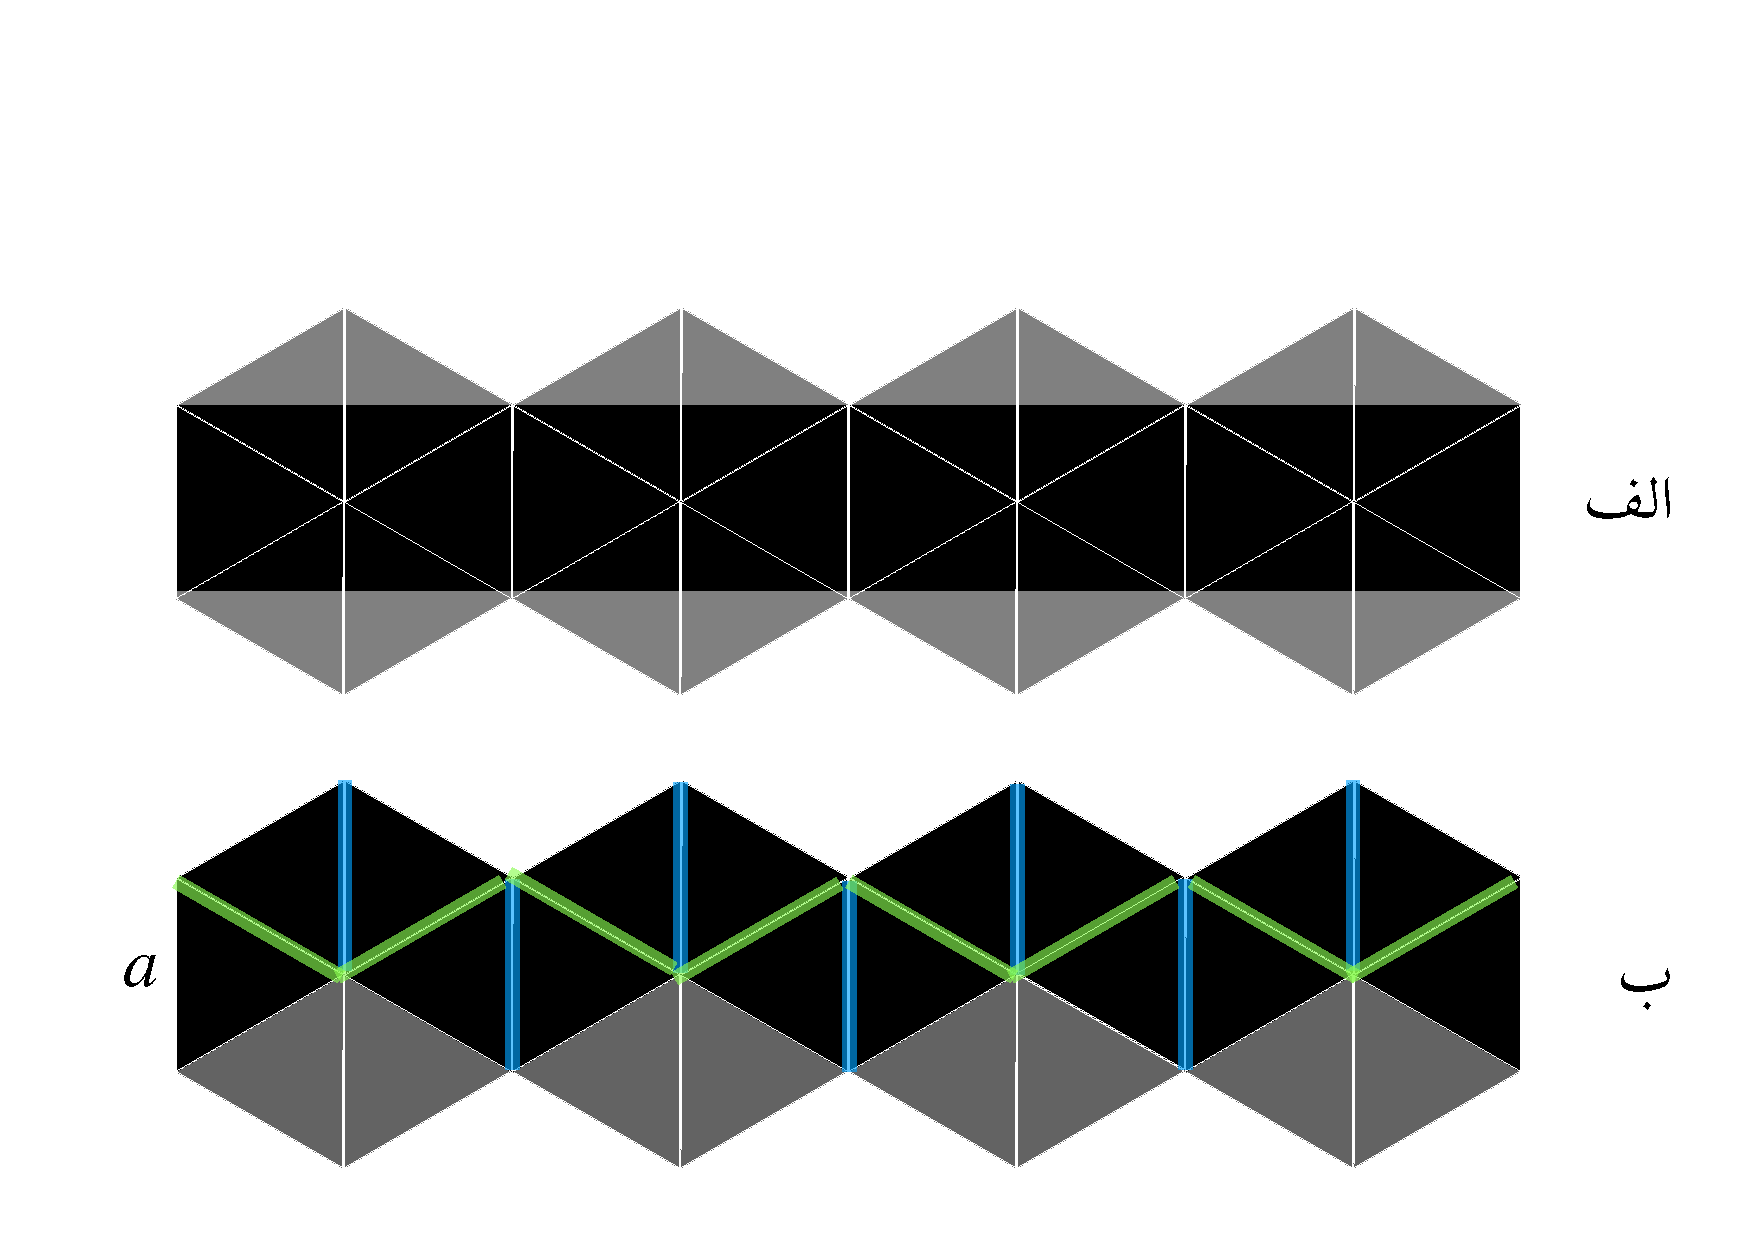
\includegraphics[width=6in]{cylindermesh.pages.pdf}
\caption{
الف، و ب، هر دو نواری از یک شبکه‌ی مثلثی را نشان می‌دهند که هر دو از تعداد یکسان مثلث تشکیل شده‌اند. 
}
\label{fig:cylindermesh}
\end{center}
\end{figure}



ژینوس استوانه برابر ۱ است در نتیجه‌ در محاسبه‌ی انرژي خمش سهمی نخواهد داشت. حال فرض کنید که سطح استوانه را با مثلث (شبکه‌ی نقاط با درجه‌ی ۶) پوشاندیم. شکل
\ref{fig:cylindermesh}
الف، چنین نواری را نشان می‌دهد. اگر فرض کنیم که مثلث‌های نصف شده در بالا و پایین نوار را جابجا کنیم تا مثلث‌های کامل تشکیل شود با شکل
\ref{fig:cylindermesh}
ب، رو برو می‌شویم. اگر این نوار را به دور یک استوانه ببندیم مثلث‌هایی که ضلع مشترک آبی رنگ دارند با یکدیگر زاویه می‌سازند در صورتی که مثلث‌هایی که اضلع مشترک  سبز دارند با یکدیگر زاویه‌ی ۱۸۰ درجه تشکیل می‌دهند. فرض کنیم که طول اضلاع مثلث‌های متساوی الاضلاع 
$a$
 باشد و نوار توسط 
 $N$
 مثلث پوشانده می‌شود. زاویه‌ی میان مثلث‌هایی که ضلع آبی مشترک دارند،
 $\pi\frac{N-2}{N}$
بوده که در نتیجه زاویه‌ی میان بردار‌های عمود به آنها،
 $\pi(1-\frac{N-2}{N})$
خواهد بود. با فرض اینکه تعداد مثلث‌ها به اندازه‌ی کافی بزرگ باشد، انرژی چنین چیدمانی

\begin{equation}
\begin{aligned}
E_{discrete}&=\epsilon_b\sum_{<\alpha,\beta>}\left[1-\cos(\theta_{\alpha,\beta})\right]\\
&=2N\epsilon_b\left[1-\cos\left(\pi(1-\frac{N-2}{N})\right)\right]\\
&=2N\epsilon_b\left[1-\left(1-\frac{1}{2}\left(\pi(\frac{2}{N}\right)^2\right)\right]\\
&=N\epsilon_b\left[\frac{\pi^2}{2}\left(\frac{2}{N}\right)^2\right]\\
&=\frac{4\pi^2}{N}\epsilon_b
\end{aligned}
\label{eq:cylinderdiscrete}
\end{equation} 
در حد 
$N$
های خیلی بزرگ معادله‌ی 
\ref{eq:cylinderdiscrete}
 و 
\ref{eq:cylindercontinuum}
باید پاسخ یکسان داشته باشند. از طرفی محیط سطح مقطع دایره‌ای استوانه با تعداد مثلث‌ها و طول ضلع آن رابطه دارد،
\begin{equation}
\begin{aligned}
2 \pi R &= \frac{N}{2}\frac{\sqrt3}{2}a\\
\frac{a}{R}&=\frac{8}{\sqrt3}\frac{\pi}{N}
\end{aligned}
\label{eq:cylinderdiscretisation}
\end{equation} 
برابر قرار دادن انرژي حد پیوسته و گسسته و جایگاذاری نسبت ضلع مثلث به شعاع استوانه از معادله بالا ما را به رابطه‌ی میان سختی خمش هلفریش و ضریب جفت شدگی مثلث‌ها می‌رساند:
\begin{equation}
\begin{aligned}
\pi\kappa\frac{a}{R}&=4\frac{\pi^2}{N}\epsilon_b\\
\pi\kappa\frac{8}{\sqrt3}\frac{\pi}{N}&=4\frac{\pi^2}{N}\epsilon_b\\
\kappa&=\frac{\sqrt{3}}{2}\epsilon_b
\end{aligned}
\label{eq:epsilonkappa}
\end{equation} 













\section{
تغییر انرژی کششی ناشی از افزودن نقطه‌ی نقص به شبکه
}
در نظریه‌ی الاستیک سطح هر تغییر شکل با یک میدان بردار جابجایی 
$u(r)=(u_1,u_2)$
نشان داده می‌شود نقطه‌ی 
$r(x,y)$
را به نقطه‌ی 
$r+u$
نگاشت می‌کند. اگر در شبکه نقص وجود نداشته باشد این نگاشت یک به یک خواهد بود. در صورتی که در شبکه دررفتگی
\LTRfootnote{dislocation}
یا نقص وجود داشته باشد هر انتگرال بسته پاد ساعتگرد که محل نقص داخل آن قرار گیرد با بردار ثابت برگر
\LTRfootnote{Burger}
برابر خواهد بود.
\cite{mitchell1961}
از آنجایی هم که بردار برگر همیشه با یکی از بردارهای شبکه برابر است، یک به یک نبودن نگاشت در حضور نقص مشکلی در فیزیک مسئله ایجاد نخواهد کرد. این بحث به زبان ریاضی شکل زیر را به خود می‌گیرد،
\begin{equation}
\begin{aligned}
&\oint_Ldu_k=\oint_L\partial_iu_kdx_i=b_k\\
&\epsilon_{li}\partial_l\partial_iu_j=b_j\delta(r-r_0)
\end{aligned}
\end{equation}
که در بالا 
$r_0$
محل نقص، و 
$b$
 بردار برگر است. در رفتگی  بر حسب میدان زاویه‌ی بین پیوندهای شبکه مشخص می‌شود، که جهت گیری در پیرامون هر اتم را مشخص می‌کند. صراحت هر نقص،
 $s$
 حول هر مسیر بسته دور نقص تعریف می‌شود. در شبکه‌ای که تقارن $n$
 تایی داشته باشد، 
 $s$ حتما ضریبی از 
 $2\pi/n$ خواهد بود.
 در این بخش شبکه‌های شش ضلعی با تقارن 
 $n=6$
و لغزش‌های کوچک
$s=\pm2\pi/6$
مورد توجه ماست. به زبان ریاضی می‌توان این جملات را به این شکل نشان داد،

 \begin{equation}
\begin{aligned}
&\oint_Ld\theta=\oint_L\partial_i\theta dx_i=s\\
&\epsilon_{ij}\partial_i\partial_i\theta=s\delta(r-r_0)
\label{eq:thetauij}
\end{aligned}
\end{equation}
با جایگذاری
\begin{equation}
\theta=\frac{1}{2}\epsilon_{ij}\partial_iu_j
\end{equation}
حال می‌خواهیم شرایط معادله‌ی 
\ref{eq:constraint}
را به صورت قید برای $\chi$
تعریف کنیم تا تضمین کند که همیشه می‌توانیم $\chi$
را به صورت جابجایی‌ها بنویسیم. برای اینکار طرفین معادله‌ی 
\ref{eq:constraint}
را در 
$\epsilon_{ik}\epsilon_{jl}\partial_k\partial_l$
ضرب می‌کنیم که نتیجه‌ی آن،
\begin{equation}
\frac{1}{Y}\nabla^4\chi=\epsilon_{ik}\epsilon_{jl}\partial_k\partial_lu_{ij}=\epsilon_{ik}\epsilon_{jl}\partial_k\partial_l\frac{1}{2}(\partial_iu_j+\partial_ju_i)
\label{eq:incompatibility}
\end{equation}
در صورتی که سمت راست معادله‌ی فوق برابر با صفر شود، می‌توان گفت که $u_{ij}$ 
سازگار است و تنها یک جواب برای میدان جابجایی وجود دارد که جواب معادله‌ی 
\ref{eq:constraint}
است. در غیر این صورت معدله‌ی 
\ref{eq:constraint}
بیش از یک جواب دارد. در نتیجه رایج است که به نام سمت راست معادله‌ی
\ref{eq:incompatibility}
را ناسازگاری
\LTRfootnote{incompatibility}
و $\epsilon_{ik}\epsilon_{jl}\partial_k\partial_l$
را عملگر ناسازگاری بنامند. می‌توانیم محاسبات معادله‌ی 
\ref{eq:incompatibility}
را به این شکل ادامه دهیم،

\begin{equation}
\begin{aligned}
\frac{1}{Y}\nabla^4\chi&=\epsilon_{ik}\epsilon_{jl}\partial_k\partial_l\frac{1}{2}(\partial_iu_j-\partial_ju_i)+\epsilon_{ik}\epsilon_{jl}\partial_k\partial_l\partial_ju_i\\
&=\epsilon_{kl}\partial_k\partial_l\theta+ \epsilon_{ik}\partial_k(\epsilon_{jl}\partial_l\partial_ju_i)\\
&=\sum_{\alpha}s_\alpha\delta(r-r_\alpha)+\sum_\beta b_i^\beta\epsilon_{ik}\partial_k\delta(r-r_\beta)
\label{eq:disclination}
\end{aligned}
\end{equation}
که $s_\alpha$
بار نقص در محل $r_\alpha$
و $b^\beta$
بردار برگر لغزش در محل $r_\beta$
را مشخص می‌کند. خط آخر معادله‌ی 
\ref{eq:disclinationX}
چگالی نقصان
$s(r)$
 را در شبکه مشخص می‌کند. در نتیجه نظریه کشسانی ۲ بعدی به معادله‌ی زیر خلاصه می‌شود،
\begin{equation}
\frac{1}{Y}\nabla^4\chi=s(r)
\label{eq:masterstretch}
\end{equation}
بدون در نظر گرفتن شرایط مرزی معادله‌ی فوق جواب یکه نخواهد داشت. فرض کنیم که یک غشای دایروی را بررسی می‌کنیم که در مرز‌ها آزاد است. در نتیجه جمع نیرو‌ها روی مرز باید صفر باشد، یعنی 
$\sigma_{rr},\sigma_{r\phi}=0$
. اگر فرض کنیم که لغزش در مرکز مختصات است، معادله‌ی 
\ref{eq:masterstretch}
به شکل زیر در می‌آید،
\begin{equation}
\frac{1}{Y}\nabla^4\chi=b_i\epsilon_{ij}\partial_j\delta(r)
\end{equation}
که به پاسخ
\begin{equation}
\chi=\frac{Y}{4\pi}b_i\epsilon_{ij}r_j\ln r
\label{eq:masterstretchsol}
\end{equation}
منجر می‌شود. البته که اگر قرار بود معدله‌ی 
\ref{eq:masterstretch}
را برای شرایط مرزی محدود حل کنیم،‌ باید جملات دیگری نیز به پاسخ 
\ref{eq:masterstretchsol}
اضافه می‌کردیم، ولی از آنجایی که این جملات در حد 
$r\rightarrow\infty$
صفر می‌شوند با این پاسخ مسئله‌ را جلو می‌بریم. حالا معادله‌ی 
\ref{eq:stress}
را بر حسب تنش می‌نویسیم،
\begin{equation}
F_s=\frac{1}{2Y}\int d^r(\nabla^2\chi)^2-\frac{1+\nu}{2Y}\int d^r\epsilon_{ik}\epsilon_{jl}\partial_k\partial_l(\partial_i\chi\partial_j\chi)
%\label{eq:masterstretchsol}
\end{equation}
با جایگذاری $\chi$ از معادله‌ی
\ref{eq:masterstretchsol}
و انتگرال گیری خواهیم داشت،
\begin{equation}
F_s=\frac{Yb^2}{8\pi}\ln\left[\frac{R}{a}\right]
%\label{eq:masterstretchsol}
\end{equation}
که انرژی حاصل از لغزش در محدوده‌ی 
$a\leq r\leq R$
در یک غشا با اندازه‌ی محدود را مشخص می‌کند. حالا معادله‌ی 
\ref{eq:masterstretch}
را برای وجود نقص در  مرکز  شبکه جلو می‌بریم.
\begin{equation}
\begin{aligned}
&\frac{1}{Y}\nabla^4\chi=s\delta(r)\\
&\chi=\frac{Ys}{8\pi}(Ar^2+r^2\ln r)
%\label{eq:disclination}
\end{aligned}
\end{equation}
بدون وجود جمله‌ی $Ar^2$
حاصل معادله کرنش بی‌نهایت در مرز خواهد بود که با آهنگ $\ln R$ بزرگ می‌شود. از آنجایی که تمام تقریب‌هایی که تا به الان استفاده شد هارمونیک بودند، این رفتار غیر قابل قبول خواهد بود زیرا که در این صورت ماده به علت کرنش زیاد از هم گسسته خواهد شد. به علت تقارن چرخش در مسئله نیز مؤلفه‌ی تنش زاویه‌دار نیز صفر  خواهد بود
\begin{equation}
\sigma_{r\phi}=-\frac{\partial}{\partial r}\left[\frac{1}{r}\frac{\partial\chi}{\partial\phi}\right]
\end{equation}
در این صورت نیاز است که در مرز مؤلفه‌ی تنش،
\begin{equation}
\sigma_{rr}=\frac{1}{r}\frac{\partial\chi}{\partial r}+\frac{1}{r^2}\frac{\partial^2\chi}{\partial \phi^2}
\end{equation}
یعنی هنگامی که $r=R$ جمله‌ی بالا صفر شود که حاصل آن تعیین کمیت $A$
است،
\begin{equation}
A=-\frac{1}{2}-\ln R
\end{equation}
حالا می‌توانیم تعریف مناسبی از تنش و انرژي سیستم را بنویسیم،
\begin{equation}
\begin{aligned}
&\chi=\frac{Ys}{8\pi}r^2\left[\ln \left(\frac{r}{R}\right)-\frac{1}{2}\right]\\
&E_s=\frac{Ys^2}{32\pi}R^2
%\label{eq:disclination}
\end{aligned}
\end{equation}



















\section{
تغییر انرژی خمش ناشی از افزودن نقطه‌ی نقص به شبکه
}
برای اینکه جابجایی خارج از صفحه را توصیف کنیم علاوه بر میدان جابجایی 
$u(r)=(u_1,u_2)$
نیاز به تابع جدید 
$f(r)$
داریم که انحراف
\LTRfootnote{deflection}
 نقاط شبکه را توصیف می‌کند یعنی تغییرات نقطه‌ی 
$(x_1,x_2,0)$
را به نقطه‌ی 
$(x_1+u_1,x_2+u_2,f)$
نگاشت می‌کند. در نتیجه انرژي کل سیستم حاصل جمع انرژی کشسانی و انرژي خمشی خواهد بود. انرژی کشسانی همچنان طبق معادله‌ی
\ref{eq:energylame}
با این تفاوت که به جای تعریف کرنش در معادله‌ی 
\ref{eq:simplestrain}
از رابطه‌ی زیر استفاده می‌کنیم
\begin{equation}
u_{ij}=\frac{1}{2}(\partial_iu_j+\partial_ju_i+\partial_if\partial_jf)
\label{eq:nonlinearstrain}
\end{equation}
در اینجا نیز همانند بخش قبلی از جملات مرتبه‌ی ۲ به بالای جابجایی صرف نظر کرده‌ایم. معمولا هنگام  مدل‌سازی صفحات تخت در حالت تغییر شکل کوچک همچنان استفاده از معدله‌ی 
\ref{eq:simplestrain}
رایج است که حاصل آن یک نظریه‌ی کاملا خطی است. در اینجا ما قصد داریم تغییر شکل‌هایی را بررسی کنیم که در آن $f$ مهم است و کمترین مرتبه‌ای که $f$ 
تاثیر خود را نشان می‌دهد مرتبه‌ی دوم است، در نتیحه کرنش را به شکل  معادله‌ی 
\ref{eq:nonlinearstrain}
قابل قبول است. انرژی خمش را طبق نظریه‌ی هلفریش
\cite{Helfrich1973}
با خمش سطح $H$
و خمش گاووسی $K$
تعریف می‌کنیم، 
\begin{equation}
F_b=\int dS\left(\frac{1}{2}\kappa H^2+\kappa_GK\right)
\end{equation}
که در اینجا 
$\kappa$
سختی خمش، 
$\kappa_G$
سختی گاووسی، و 
$dS$
عنصر سطح است. خمش بر حسب 
$f$
 به شکل زیر محاسبه می‌شوند،
\begin{equation}
\begin{aligned}
H&=\nabla\cdot\left[\frac{\nabla f}{\sqrt{1+|\nabla f|^2}}\right],\\
K&=\frac{\det(\partial_i\partial_jf)}{\left(1+|\nabla f|^2\right)^2}
\end{aligned}
\end{equation}
برای تغییر شکل‌های کوچک می‌توانی از تقریب زیر استفاده کنیم،
\begin{equation}
\begin{aligned}
H&\approx\nabla^2f\\
K&\approx \det(\partial_i\partial_jf)=-\frac{1}{2}\epsilon_{ik}\epsilon_{jl}\partial_k\partial_l(\partial_if\partial_jf)
\end{aligned}
\end{equation}
با جایگذاری روابط بالا می‌توانیم انرژي خمش را بازنویسی کنیم،
\begin{equation}
F_b\approx\frac{1}{2}\kappa\int d^2r(\nabla^2 f)^2+\frac{1}{2}\kappa_G\int d^2r\epsilon_{ik}\epsilon_{jl}\partial_k\partial_l(\partial_if\partial_jf)
\label{eq:bendingenergyequ}
\end{equation}
حالا با مشتق‌گیری نسبت به $u$ و $f$
می‌توانیم مانند بخش قبل معادلاتی که به تعریف تنش می‌انجامد را تعریف کنیم
\begin{equation}
\begin{aligned}
\kappa\nabla^4f&=\partial_i(\sigma_{ij}\partial_jf)\\
\partial_i\sigma_{ij}&=0
\end{aligned}
\end{equation}
که در بالا رابطه‌ی بین تانسور تنش و تانسور غیر خطی کرنی مشابه معادله‌ی 
\ref{eq:stress}
تعریف شده است. حالا مشابه مراحلی که منجر به معادله‌ی 
\ref{eq:disclination}
شد عمل کرده و به رابطه‌ی زیر می‌رسیم،

\begin{equation}
\frac{1}{Y}\nabla^4\chi-\frac{1}{2}\epsilon_{ik}\epsilon_{jl}=\sum_\alpha s_\alpha\delta(r-r_\alpha)+\sum_\beta b_i^\beta\epsilon_{ik}\partial_k\delta(r-r_\beta)
\end{equation}
و در نهایت می‌توانیم یک سیستم معادلا کامل بنویسیم،
\begin{equation}
\begin{aligned}
&\kappa\nabla^4f+\epsilon_{ik}\epsilon_{jl}\partial_k\partial_l(\partial_i\chi\partial_jf)=0\\
&\frac{1}{Y}\nabla^4\chi=s(r)-K(r)
\end{aligned}
\end{equation}
و همانند قسمت قبل $s(r)$ چگالی نقص و 
$k(r)$
خمش گاووسی است. نقش خمش گاووسی به صورت کم کردن تنش در اینجا ظاهر می‌شود. از آنجایی که انتگرال خمش گاووسی به انتگرال روی محیط می‌تواند کاهش پیدا کند بر روی فیزیک روی سطح مسئله تاثیر نمی‌گذارد بلکه تاثیر خود را روی شرایط مرزی نشان می‌دهد. پس به قیود 
$\sigma_{rr},\sigma_{r\phi}=0$
باید قیود زیر را نیز اضافه کنیم،
\begin{equation}
\begin{aligned}
&\frac{\kappa}{\kappa_G}\nabla^2f+\left[\frac{1}{r}\frac{\partial f}{\partial r}+\frac{1}{r^2}\frac{\partial^2 f}{\partial\phi^2}\right]=0\\
&\frac{\kappa}{\kappa_G}\frac{\partial}{\partial r}\nabla^2f-\frac{1}{r}\frac{\partial}{\partial r}\frac{1}{r}\frac{\partial^2 f}{\partial\phi^2}=0
\end{aligned}
\end{equation}
که بر روی مرز دایروی ارضاء می‌شوند. اگر بسط بالا را باز کنیم معادلات شکل زیر را به خود می‌گیرند،

\begin{equation}
\begin{aligned}
&\kappa\nabla^4f=\frac{\partial^2\chi}{\partial y^2}\frac{\partial^2f}{\partial x^2}+\frac{\partial^2\chi}{\partial x^2}\frac{\partial^2f}{\partial y^2}-\frac{\partial^2\chi}{\partial x\partial y}\frac{\partial^2f}{\partial x\partial y},\\
&\frac{1}{Y}\nabla^4\chi+\frac{\partial^2f}{\partial x^2}\frac{\partial^2f}{\partial y^2}-\left[\frac{\partial^2f}{\partial x\partial y}\right]^2=\sum_\alpha s_\alpha \delta(r-r_\alpha)+\sum_\beta b_i^\beta \epsilon_{ik}\partial_k\delta(r-r_\beta)
\end{aligned}
\end{equation}
در صورتی که هیچ نقصی در شبکه وجود نداشته باشد و جملات شامل دلتای دیراک را برابر با صفر قرار دهیم همان معادله‌ی کارمن
\LTRfootnote{Kármán}
 را بدس می‌آوریم. این معدلات غیر خطی به راحتی قابل حل نیستند. سعی می‌کنیم این معادلات را برای حالت خیلی ساده شده‌ای که شامل یک نقص در مرکز شبکه‌ای که نسبت به مرکز تقارن دایره‌ای داشته باشد، حل کنیم. برای فواصل دور از نقطه‌ی نقص،‌ معادلات به شکل زیر در می‌آید،

\begin{equation}
\begin{aligned}
&\kappa\nabla^4f=\frac{1}{r}\frac{d}{dr}\left[\frac{d\chi}{dr}\frac{df}{dr}\right],\\
&\frac{1}{Y}\nabla^4\chi+\frac{1}{2r}\frac{d}{dr}\left[\frac{df}{dr}\right]^2=0
\end{aligned}
\end{equation}

که گرادیان به شکل زیر در نظر گرفته شده،
\begin{equation}
\nabla^2=\frac{1}{r}\frac{d}{dr}r\frac{d}{dr}
\end{equation}
. حدس می‌زنیم جواب معادلات به شکل زیر باشد،


\begin{equation}
\begin{aligned}
&\chi=-\kappa\ln\left[\frac{r}{a}\right]\\
&f=\pm\left[\frac{s}{\pi}\right]^{\frac{1}{2}}r
\end{aligned}
\end{equation}
. پس می‌توانیم بردار جابجایی را با کمک معادله‌ی 
\ref{eq:nonlinearstrain}
بنویسیم. 

\begin{equation}
\begin{aligned}
&u_x=-\frac{s}{2\pi}y\phi-\frac{s}{2\pi}x+\frac{\kappa(1+\sigma)}{Y}\frac{x}{r^2}\\
&u_y=\frac{s}{2\pi}x\phi-\frac{s}{2\pi}y+\frac{\kappa(1+\sigma)}{Y}\frac{y}{r^2}
\end{aligned}
\end{equation}
که در اینجا
$\frac{y}{x}=\tan\phi$
. در نهایت با جایگذاری پاسخ حدسی در معادله‌ی
\ref{eq:bendingenergyequ}
به فرم انرژی زیر می‌رسیم.
\begin{equation}
E_{bending}= s\kappa\ln\left[\frac{R}{a}\right]
\end{equation}







\section{
بیولوژی غشا و ساختار آن
}

\section{
اطلاعاتی که باید اضافه بشه
}
در این بخش مقاله‌هایی  که استفاده کردم و هنوز اضافه نشده را می‌ذارم.

این مقاله همه جا رفرنس داده شده که نشون دادن که ساختار ایکوسهیدرال و نواقص چه روابط ریاضی دارن.
\cite{CasparKlug1962}
نلسون در اینجا با جزئیات زیاد شکل ویروس و گاما را بررسی می‌کند.
\cite{nelsonPRE2003}
در این مقاله نحوه‌ی تاثیر گاما بر شکل وسیکل بررسی شده است. این مقاله بر اساس کارهای نلسون در این زمینه‌ است.
\cite{gammaPRE2005}

در این مقاله نلسون کلوئید در قطره‌های کروی آب قرار می‌دهد و توزیع نقص روی سطح را بررسی می‌کند.
\cite{NelsonScience2003}
و  تئوری آن نیز در این مقاله‌ محاسبه ‌شده
\cite{NelsonPRB2000}
اینجا اولین جایی است که  من پیدا کردم که نشان می‌دهد ضریب تبدیل جفت شدگی بردارهای عمود بر مثلث‌ها به سختی خمشی برای  شکل  کلی کره و استوانه متفاوت است. 
\cite{GompperKroll1996}












\section{
بررسی مدل گومپر-کرول
}
همانند بخش‌های دیگر فیزیک مانند دینامیک شاره‌ها و نظریه‌ی رسانایی در فلزات، نظریه‌ی پوسته‌های نازک می‌خواهد فیزیک اختلال‌های کُند را بر حسب چند پارامتر ماکروسکوپیک بیان کند. البته که بارها نشان داده شده که چنین نظریه‌هایی به شکل‌ جالبی فروپاشی می‌کنند. مانند با توجه به نظریه جفت شدن مُود‌ها و نظریه باز به هنجارش، افت و خیز‌ها گرمایی باعث می‌شوند که وشکسانی برشی
\LTRfootnote{shear viscosity}
شاره‌های تراکم ناپذیر در ۲ بعد به صورت لوگاریتمی با افزایش اندازه سیستم به بی نهایت میل می‌کند 
\cite{gomppernelson2012}
. غیر خطی شدن رفتار در مورد پوسته‌ها و صفحه‌های نازک نیز اتفاق می‌افتد. افت و خیز گرمایی می‌توانند بر ساختار پوسته‌هایی میکرونی به شدت تاثیر بگذارند زیراکه انرژی خمشی لازم برای بیشتر تغییر شکل‌های پوسته‌های خیلی نازک که زخامت آنها در مقیاس نانومتر است، حدود $k_BT$ است که در اینجا $k_B$ ثابت بولتزمن و
$T$
دماست. مکانیک آماری غشاها و صفحات تخت در گذشته بسیار دقبق مورد مطالعه قرار گرفته. در این سیستم‌ها نشان داده شده‌است که افت و خیز گرمایی در غشاهای تخت باعث می‌شود که مدول کشسانی درون صفحه‌ای
\LTRfootnote{in-plane}
 تابع اندازه‌‌ی سیستم باشد و در اندازه‌های بزرگ به سمت صفر میل کند در حالی که مدول خمشی به بی‌نهایت میل می‌کند. این پدیده‌های ناهنجار ناشی از جفت شدگی غیر خطی میان تغییر شکل‌های خارج از صفحه‌ای (عمود بر صفحه) و تنش‌هایی داخل صفحه‌ی که ایجاد می‌کنند که هنگام تغییر شکل خارج از صفحه از مرتبه‌ی دوم هستند. حتی اطلاعات کمتری در مورد تاثیر افت و خیز گرمایی بر غشا‌های کروی موجود است (شکل 
 \ref{fig:mem1}
)
ولی جفت شدگی بین تغییر شکل‌های روی سطح و عمود بر سطح با یکدیگر تفاوت دارند. به علت وجود هندسه‌ی بسته‌ی غشاهای شبه کروی تغییر شکل حتما همراه با ایجاد کشش در سطح است. در نتیجه جابجایی عمود بر سطح به شکل جملات مرتبه‌ی اول در تنش موازی با صفحه ظاهر می‌شوند. در نتیجه جفت‌ شدگی‌های غیر خطی متفاوت با غشای تخت ایجاد می‌‌شود.

انرژی کشسانی تغییر شکل غشا به شعاع
 $R$ 
با نظریه‌ی پوسته‌های نازک کم عمق مدل‌سازی می‌شود. با این روی‌کرد صحبت از فرورفتیگی‌ها یا برآمدگی‌هایی است که نسبت به بخش مورد مطالعه کوچک هستند. جابجایی درون صفحه با فنون دو مولفه‌ای 
$u_i(\boldsymbol{x})$ 
پارمتری‌سازی شده و جابجایی‌های عمود بر سطح با میدان 
$f(\boldsymbol{x})$
در دستگاه مختصات
$\boldsymbol{x}=(x_1,x_2)$
موازی سطح تعریف می‌‌شود. ما فرض می‌کنیم که تمام غشای مورد بررسی دارای خواص کشسانی هماهنگ در همه جای سطح است در نتیجه می‌توانیم تاثیر ۱۲ نقطه نقصی که به ناچار بر روی سطح کره‌ی مثلث بندی شده ایجاد می‌شود را ناچیز در نظر بگیریم.
















\section{محاسبه‌ی اندازه افت و خیز روی کره}
در این بخش نحوه‌ی اندازه‌ی دامنه‌ی افت و خیزهایی که بر روی سطح کره اینجاد می‌شود را اندازه‌گیری می‌کنیم. 
\cite{safran1983}
فرض می‌کنیم که انرژی خمش کُره به شکل زیر تعریف می‌شود
\begin{equation}
E_{b}=\frac{1}{2}\kappa\int dS\left(H-H_0\right)^2
\end{equation}
 که در اینجا 
 $\kappa$
 سختی خمش و
 $H$
و 
$H_0$
به ترتیب خمش و خمش ذاتی سطح کروی است. خمش ذاتی به شکل 
$H_0=2/r_s$
و خمش سطح به شکل
\begin{equation}
H=\left(\frac{1}{r_1}+\frac{1}{r_2}\right)=\frac{\nabla\cdot\hat n}{2}
\end{equation}
تعریف می‌شود. در معادلات بالا 
$r_s$
شعاع خمش ذاتی و 
$r_1$ و $r_2$
شعاع‌های پایه‌ای خمش
\LTRfootnote{princople curvature radii}
و $\hat n$ بردار عمود بر سطح است. در نتیجه انرژی خمش را به شکل زیر باز نویسی می‌کنیم
\begin{equation}
E_{b}=\frac{1}{8}\kappa\int dS\left(\nabla\cdot\hat n-\frac{2}{r_s}\right)^2
\label{eq:ebforsubstitution}
\end{equation}
سطح تقریبا کروی که مرکز آن در مبدا مختصات وجود دارد را به شکل زیر تعریف می‌کنیم
\begin{equation}
R(r)= r-r_0\left[1+g(\theta,\phi)\right]=0
\label{eq:radiusdef}
\end{equation}
. در این معادله $r_0$ شعاع متوسط کره است که $g$
\begin{equation}
g(\theta,\phi)=\sum_{\ell,m}u_{\ell m}Y_{\ell m} (\theta,\phi)
\label{eq:gdef}
\end{equation}
اختلاف شعاع هر نقطه از شعاع متوسط است که با هماهنگ‌های کروی، $Y_{\ell m}$، نشان داده شده. بردار عمود در هر نقطه از سطح کره را می‌توانیم به شکل زیر محاسبه کنیم
\begin{equation}
\hat n = \frac{\nabla R(r)}{|\nabla R(r)|}= \frac{\hat r-\frac{r_0}{r}g_\theta \hat\theta-\frac{r_0}{r\sin\theta}g_\phi\hat\phi }{\sqrt{1+\left(\frac{r_0}{r}g_\theta\right)^2+\left(\frac{r_0}{r\sin\theta}g_\phi\right)^2 }}
\end{equation}
که در اینجا برای ساده سازی از
$g_\theta=\partial/\partial\theta g$
و
$g_\phi=\partial/\partial\phi g$
استفاده شده‌است و محاسبات در دستگاه مختصات کروی انجام شده‌است.
جهت یادآوری،
\begin{equation}
\begin{aligned}
&\nabla f =\frac{\partial}{\partial r}f\hat r + \frac{1}{r} \frac{\partial}{\partial\theta}f\hat\theta+ \frac{1}{r\sin\theta} \frac{\partial}{\partial\phi}f\hat\phi\\
&\nabla\cdot \vec A =\frac{1}{r^2}\frac{\partial}{\partial r}(r^2A_r)+ \frac{1}{r\sin\theta} \frac{\partial}{\partial\theta}(A_\theta\sin\theta)+ \frac{1}{r\sin\theta} \frac{\partial}{\partial\phi}A_\phi\\
&\nabla^2f =\frac{1}{r^2}\frac{\partial}{\partial r}\left(r^2\frac{\partial}{\partial r}f\right)+ \frac{1}{r^2\sin\theta} \frac{\partial}{\partial\theta}\left(\sin\theta\frac{\partial}{\partial\theta}f\right)+ \frac{1}{r^2\sin^2\theta} \frac{\partial^2}{\partial\phi^2}f
\end{aligned}
\end{equation}
از این پس محاسبات را تنها تا مرتبه‌ی دوم نسبت به $g$ 
انجام خواهیم داد. در نتیجه بردار عمود بر سطح را به این شکل بازنویسی می‌کنیم،
\begin{equation}
\hat n \simeq\left\{1-\frac{1}{2}\left[\left(\frac{r_0}{r}g_\theta\right)^2+\left(\frac{r_0}{r\sin\theta}g_\phi\right)^2 \right]\right\}^{-\frac{1}{2}}\left( \hat r-\frac{r_0}{r}g_\theta \hat\theta-\frac{r_0}{r\sin\theta}g_\phi\hat\phi \right)
\end{equation}
حالا می‌توان دیورژانس را به ترتیب زیر محاسبه کرد،
\begin{equation}
\begin{aligned}
&\nabla\cdot\hat n \simeq \frac{2}{r}+\frac{1}{r\sin\theta}\frac{\partial}{\partial\theta}\left(-\frac{r_0}{r}g_\theta\sin\theta\right)+\frac{1}{r\sin\theta}\left(-\frac{r_0}{r\sin\theta}g_\phi\right)\\
&=\frac{2}{r}\left[1-\frac{r_0}{2r}\left(\frac{1}{\sin\theta}\frac{\partial}{\partial\theta}g_\theta\sin\theta+\frac{1}{\sin^2\theta}g_{\phi\phi}\right)\right]
\label{eq:divn}
\end{aligned}
\end{equation}
با در نظر گرفتن تعریف عملگر اندازه حرکت زاویه‌ای 
\begin{equation}
L^2=-\frac{1}{\sin\theta}\frac{\partial}{\partial\theta}\left(\sin\theta\frac{\partial}{\partial\theta}\right)-\frac{1}{\sin^2\theta}\left(\frac{\partial^2}{\partial\phi^2}\right)
\end{equation}
می‌توانیم معادله‌ی
\ref{eq:divn}
را به شکل زیر بازنویسی کنیم،
\begin{equation}
\nabla\cdot\hat n =\frac{2}{r}\left[1+\frac{r_0}{2r}L^2g\right]
\label{eq:divnL2}
\end{equation}
همچنین انتگرال عنصر سطحی را نیز می‌توان به ترتیب زیر تعریف کرد و تا حد تقریب مرتبه‌ی دوم رد $g$ جلو رفتچ
\begin{equation}
dS=r^2d\Omega\left[1+\frac{r_0^2}{2r^2}\left(g_\theta^2+\frac{g_\phi^2}{\sin^2\theta}\right)\right]=r^2d\Omega\left(1+\frac{r_0^2}{2r^2}gL^2g\right)
\label{eq:dsL2}
\end{equation}
حال کافی است که جملات بالا را در معادله‌ی \ref{eq:ebforsubstitution} جایگذاری کنیم،
\begin{equation}
E_b=\frac{1}{8}\kappa\int r^2d\Omega\left(1+\frac{r_0^2}{2r^2}gL^2g\right)\left[\frac{2}{r}\left(1+\frac{r_0}{2r}L^2g\right)-\frac{2}{r_s}\right]^2
\label{eq:ebcalc1}
\end{equation}
 $2/r$ را از جملات داخل کروشه فاکتور گرفته سپس جملات 
 \ref{eq:ebsubs}
 را در معادله‌ی
 \ref{eq:ebcalc1}
 جایگذاری می‌کنیم‌. در نتیجه انرژی به شکل زیر تعریف می‌شود،
\begin{equation}
\begin{aligned}
&\tilde{g}=\frac{1}{2}L^2g\\
&r=r_0(1+g)\\
&\frac{r_0}{r}\simeq 1-g
\label{eq:ebsubs}
\end{aligned}
\end{equation}


\begin{equation}
E_b=\frac{1}{2}\kappa\int d\Omega\left[1+\tilde gg(1-g)^2\right]\left[1+\tilde g(1-g)-\frac{r_0}{r_s}(1+g)\right]^2
\end{equation}
پس از انجام عملیات جبری و حفظ جملات تا مرتبه‌ی دوم نسبت به $g$
معادله‌ی انرژی به شکل زیر در می‌آید
\begin{equation}
\begin{aligned}
&E_b=\frac{1}{2}\kappa\int d\Omega\left[1-2\frac{r_0}{r_s}+\left(\frac{r_0}{r_s}\right)^2+\tilde gg -2\frac{r_0}{r_s}\tilde gg+\left(\frac{r_0}{r_s}\right)^2\tilde gg\right.\\
&\left.+\tilde g^2-2\tilde gg +\left(\frac{r_0}{r_s}\right)^2g^2+2\left(\frac{r_0}{r_s}\right)^2g+2\tilde g-2\frac{r_0}{r_s}g-2\frac{r_0}{r_s}\tilde g\right]
\end{aligned}
\end{equation}
پس از فاکتورگیری و مرتب سازی شکل در می‌آید
\begin{equation}
E_b=\frac{1}{2}\kappa\int d\Omega\left[\left(1-\frac{r_0}{r_s}\right)^2(1+\tilde gg)+\tilde g(\tilde g-2g)+\left(\frac{r_0}{r_s}\right)^2g^2\right]
\label{eq:ebfinal}
\end{equation}
از آنجایی که در معادله‌ی
\ref{eq:radiusdef}
افت و خیز شعاع را نسبت به شعاع متوسط تعریف کردیم، انتگرال جملات مرتبه‌ی اول $g$ روی سطح کره برابر با صفر خواهد شد، این جملات از معادله‌ی 
\ref{eq:ebfinal}
حذف شده‌اند. فرض کنیم که سطح مورد بررسی ترجیه خمش نداد و حالت کمینه انرژی آن زمانی است که سطح تخت باشد، در این صورت با $r_s\rightarrow\infty$ انرژی به شکل زیر تغییر خواهد کرد:
\begin{equation}
E_b=\frac{1}{2}\kappa\int d\Omega\left(1-g\tilde g+\tilde g^2\right)
\label{eq:ebfinalnors}
\end{equation}
حال با جایگذاری معادله‌ی
\ref{eq:gdef}
و $\tilde g=(1/2)L^2g$ در معادله‌ی بالا انرژی را محاسبه می‌کنیم.
\begin{equation}
\begin{aligned}
&E_b=\frac{1}{2}\kappa\int d\Omega\left[1-g\frac{1}{2}L^2g+\frac{1}{4}\left(L^2g\right)^2\right]\\
&=\frac{1}{2}\kappa\int d\Omega\left[1-\frac{1}{2}\sum_{\ell',m'}u_{\ell' m'}Y_{\ell' m'} (\theta,\phi)\sum_{\ell,m}u_{\ell m}L^2Y_{\ell m} (\theta,\phi)+\frac{1}{4}\left(\sum_{\ell,m}u_{\ell m}L^2Y_{\ell m} (\theta,\phi)\right)^2\right]\\
&=2\pi \kappa+\frac{1}{8}\kappa\sum_{\ell,m}|u_{\ell m}|^2\left[\ell^2(1+\ell)^2-2\ell(1+\ell)\right]\\
&=2\pi\kappa+\frac{1}{8}\kappa\sum_{\ell,m}|u_{\ell m}|^2\ell(\ell+1)(\ell-1)(\ell+2)
\end{aligned}
\end{equation}
با توجه به اصل همپاری انرژی می‌توانیم انرژی داریم،


































\section{میدان و تنش در نظریه پوسته‌ی کم عمق}
در این قسمت ما طبق روش کویتر
\LTRfootnote{Koiter}
و
\LTRfootnote{Heijden}
هیدن
پیش می‌‌رویم
\cite{Heijden2008WTK}
. بخشی از کره که دچار فرورفتگی کوچکی شده را در نظر می‌گیریم و دستگاه مختصات دکارتی 
$(x_1,x_2)$
را طوری تعریف می‌کنیم که در مبدا بر قسمت بدون ناهمواری از کره مماس است (شکل 
\ref{fig:nelson_figs1}
). در نتیجه مرکز کره بر روی محور 
$z$
خواهد بود. می‌توان کره را با فاصله نقاط آن از صفحه‌ی مختصات پارامتری سازی کرد:
\begin{equation}
Z(x_1,x_2) = R\left(1-\sqrt{1-\frac{x_1^2}{R^2}-\frac{x_2^2}{R^2}}\right)
\label{eq:nelsonS1}
\end{equation}
\begin{figure}[h]
\begin{center}
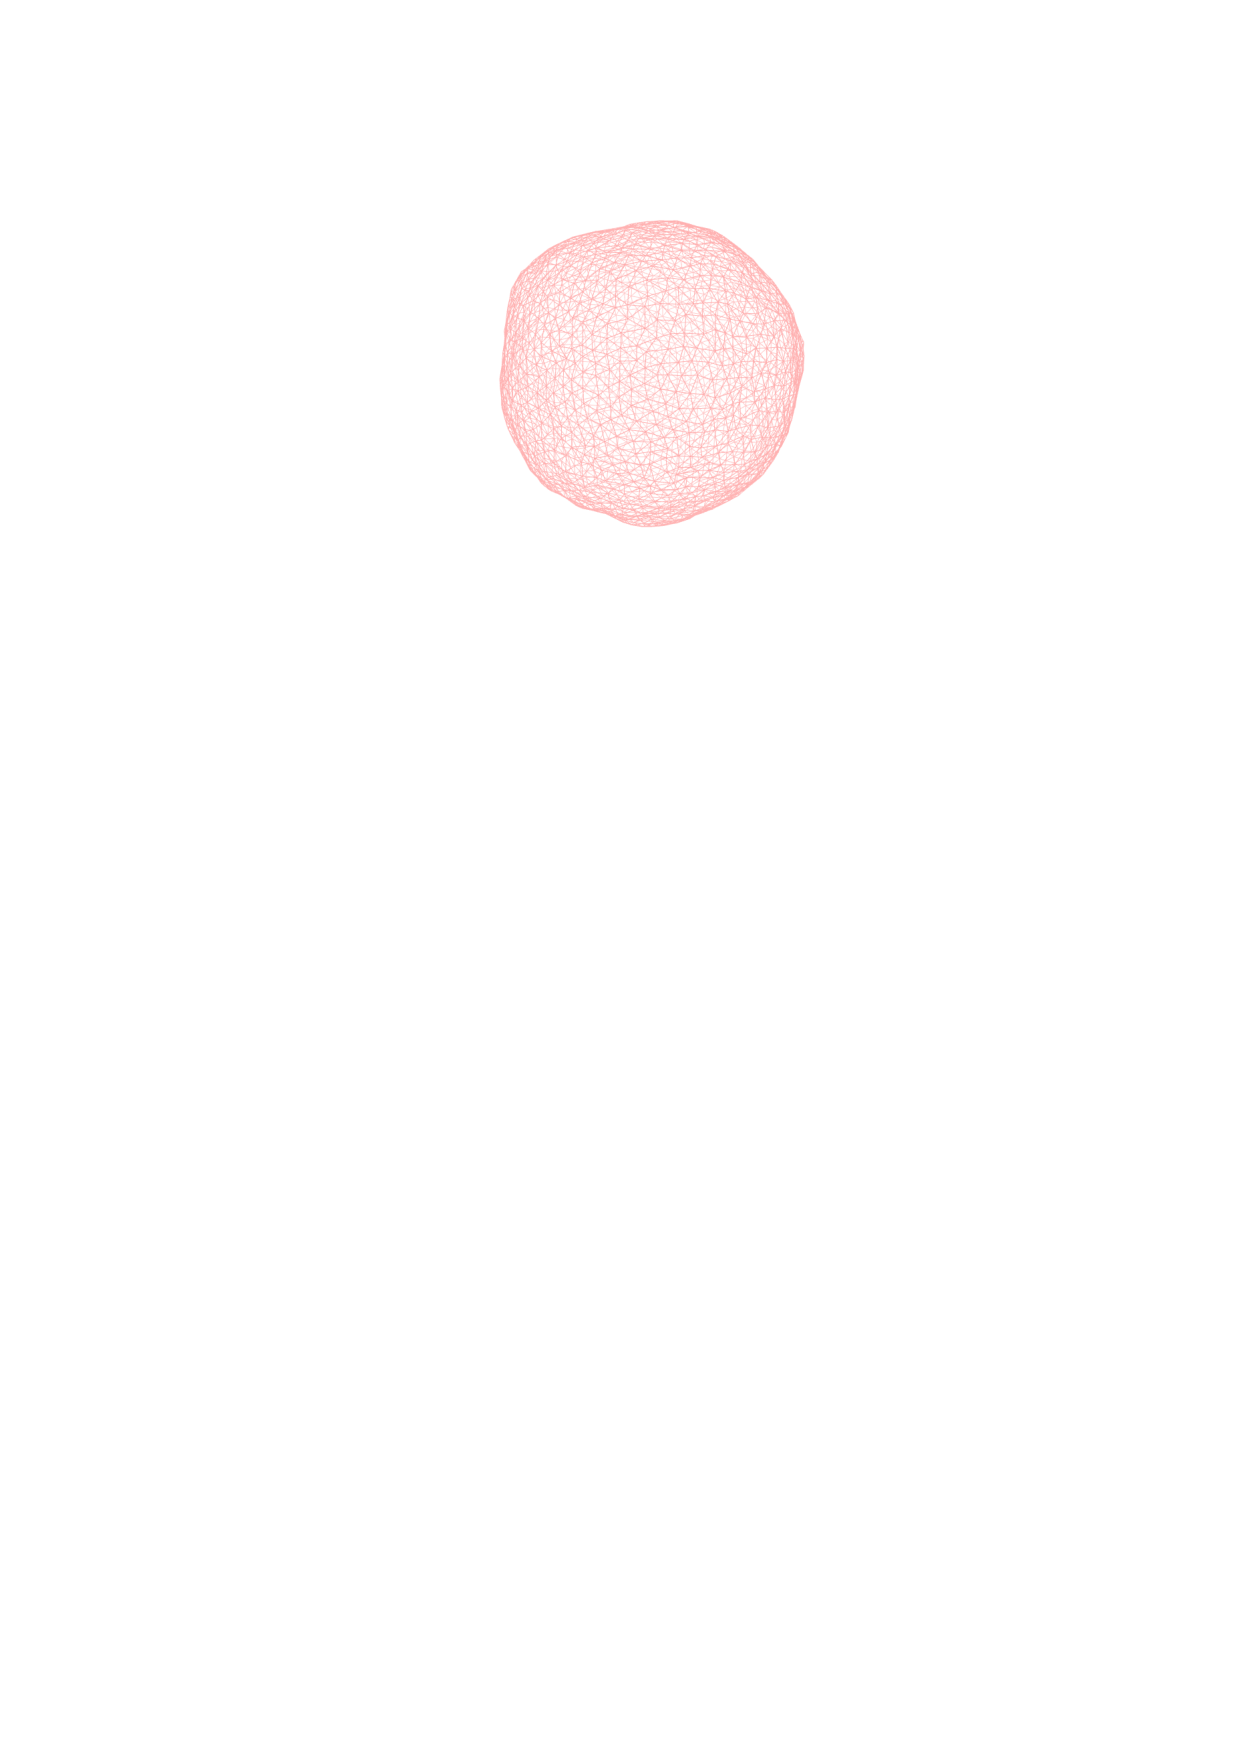
\includegraphics[width=4in]{mem_sim1}
\caption{
غشا با هندسه‌ی کروی.
}
\label{fig:mem1}
\end{center}
\end{figure}
\begin{figure}[h]
\begin{center}
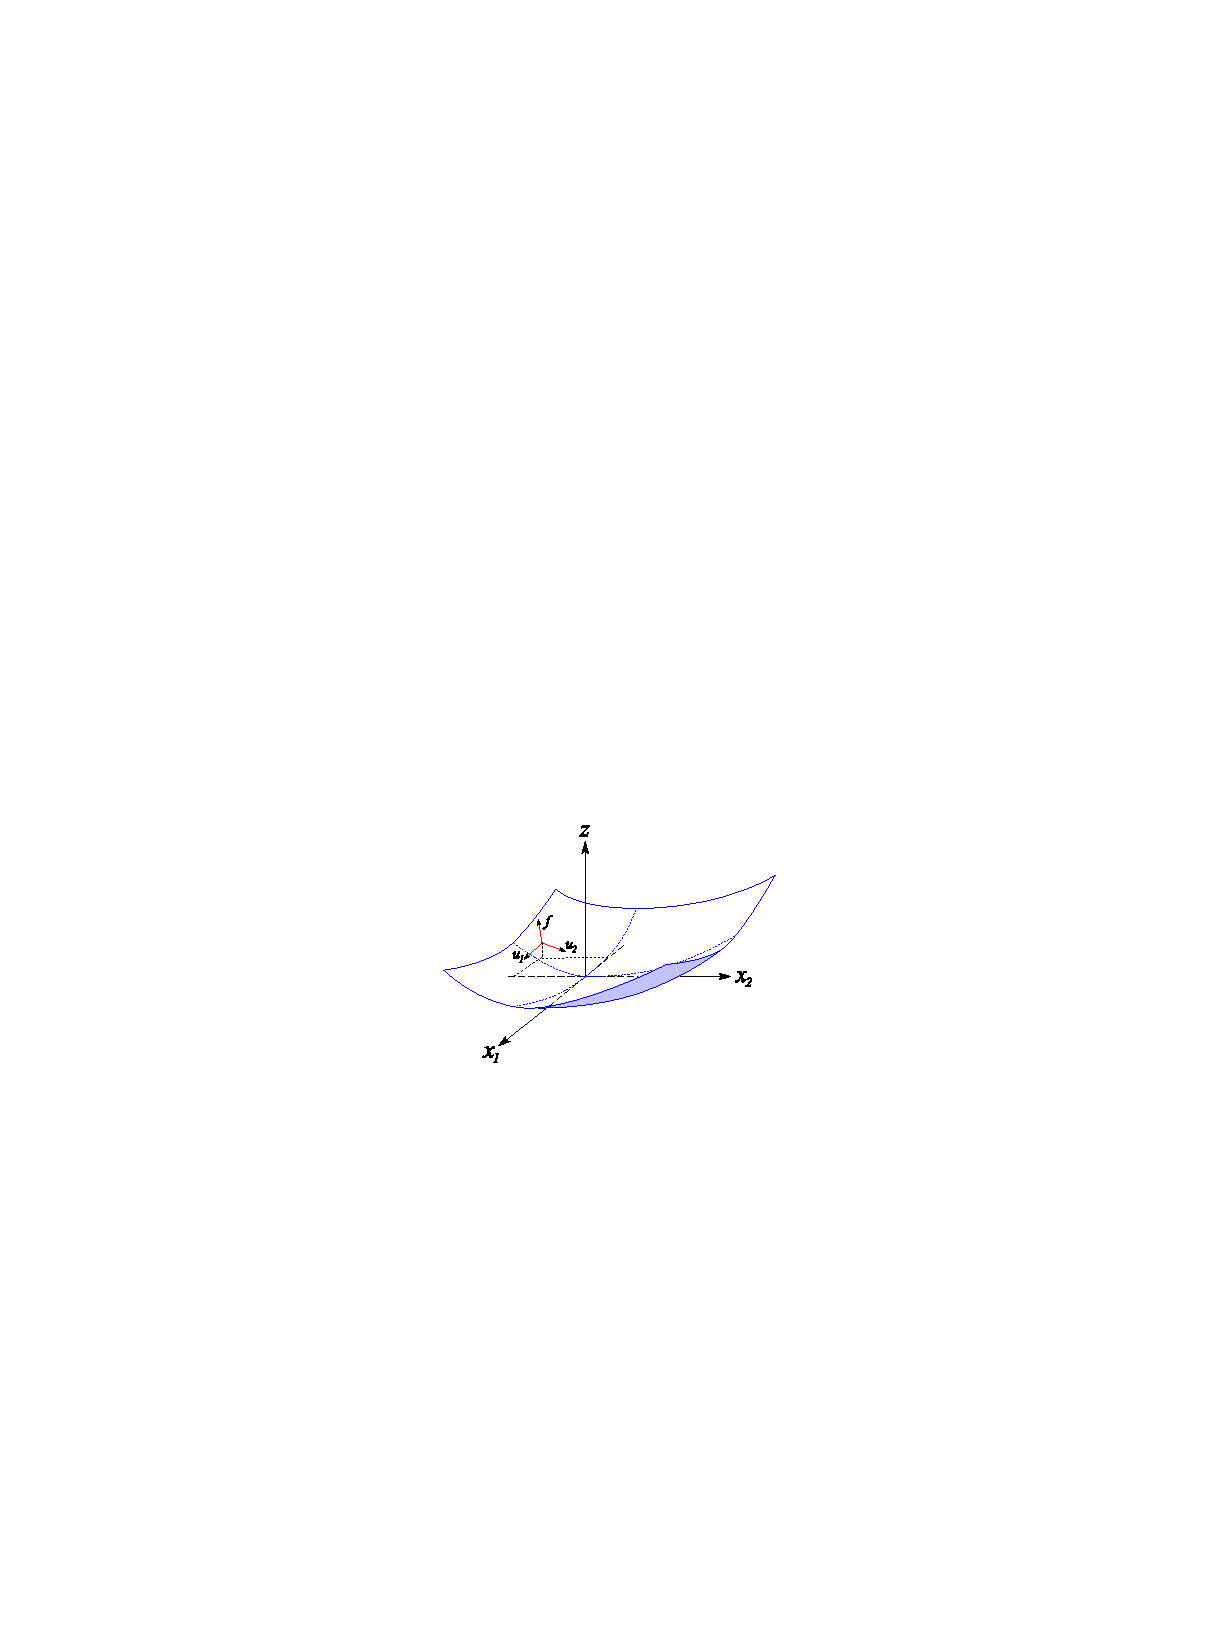
\includegraphics[width=4in]{nelsonS1}
\caption{
مبدا مختصات مماس به بخشی از کره‌ی بدون تغییر شکل.ٓ
}
\label{fig:nelson_figs1}
\end{center}
\end{figure}

که در اینجا 
$z=Z()z_1,x_2)$
نقاط روی کره در حالت بدون اختلال را مشخص می‌کند. در نظریه پوسته‌ی کم عمق
\cite{nelsonJPhysFrance1987}
 فرض می‌شود که محل بررسی به اندازه‌ای کوچک است که شیب‌های 
$\partial_1Z\sim x_1/R$
و 
$\partial_2Z\sim x_2/R$
اندازه‌گیری شده نسبت به صفحه‌ی 
$(x_1,x_2)$
کوچک هستند. در نتیجه می‌توان معادله‌ی بالا رو به شکل زیر ساده کرد:
\begin{equation}
Z(x_1,x_2) \approx \frac{x_1^2+x_2^2}{2R}
\label{eq:nelsonS2}
\end{equation}
در نتیجه تمام تغییر شکل‌های پوسته از این حالت را می‌توان بر حسب جابجایی‌های عمود بر صفحه‌
 $f(x_1,x_2)$
و جابجایی های مماس بر صفحه 
$u_1(x_1,x_2)$
و
$u_2(x_1,x_2)$
که به ترتیب جابجایی در راستای محورهای 
$x_1$
و
$x_2$
را مشخص می‌کنند، تعریف کرد. بنابراین با توجه به میدان‌های تعریف شده، نقطه‌ی 
$(x_1,x_2,Z(x_1,x_2))$
در حالت بدون جابجایی در مرتبه‌ی اول به نقطه‌ی 
$(x_1+u_1-f\partial_1Z,x_2+u_2-f\partial_2Z,Z+f)$
منتقل می‌شود که در اینجا 
$\partial_iZ=x_i/R$
است. تانسور کرنش با توجه رابطه‌ی میان اندازه‌ی یک عنصر خط در حالت تغییر حالت داده شده
$ds'$
و خط متناظر آن در حالت کاملا کروی تعریف می‌شود:
\begin{equation}
(ds')^2=ds^2+2u_{ij}dx_idx_j
\label{eq:nelsonS3}
\end{equation}
در نتیجه با صرف نظر از مشتق‌های مرتبه‌های بالاتر می‌توان تانسور کرنش را تعریف کرد،
\begin{equation}
u_{ij}=\frac{1}{2}(\partial_iu_j+\partial_ju_i+\partial_if\partial_jf)-\delta_{ij}\frac{f}{R}
\label{eq:nelsonS4}
\end{equation}
در نتیجه انرژی کششی به شکل زیر تعریف خواهد شد
\begin{equation}
G_s=\frac{1}{2}\int dS\left[2\mu u_{ij}^2+\lambda u_{kk}^2\right]
\label{eq:nelsonS5}
\end{equation}
  که در اینجا 
$\lambda$
و
$\mu$
ضرایب لامه
\LTRfootnote{Lamé}
بوده و 
$dS$
عنصر مساحت است. همچنین انرژی هلفریش
\LTRfootnote{Helfrish}
را نیز در برای تغییرات خمشی پوسته در نظر می‌گیریم
\cite{Helfrich1973}.
\begin{equation}
G_b=\frac{1}{2}\int dS\left[\kappa(H-H_0)^2+\bar\kappa K\right]
\label{eq:nelsonS6}
\end{equation}
  که در اینجا 
$\kappa$
سختی خمشی، 
$H$
خمش متوسط (یا رد
\LTRfootnote{trace}
تانسور خمش)،
$H_0$
خمش ذاتی غشا،
$\bar\kappa$
مدول خمشی زینی،
و
$K$
دترمینان تانسور خمش است . با توجه به نظریه گاوس و بونه
\LTRfootnote{Gauss-Bonnet}
این انتگرال فقط یک عدد ثابت است که به انرژی آزاد سیستم اضافه می‌شود. در نتیجه از الان به بعد آن را در نظر نمی‌گیریم. همچنین فرض می‌کنیم که غشا خمش ذاتی ندارد. در نتیجه در قسمت کم عمق پوسته خمش موضعی بر حسب 
$Z(x_1,x_2)$
و 
$f(x_1,x_2)$
به شکل زیر محاسبه می‌شود:
\cite{Helfrich1973}.
\begin{equation}
H =\nabla^2(Z+f)=\frac{2}{R}+\nabla^2f
\label{eq:nelsonS7}
\end{equation}
که 
$\nabla^2=\partial_{11}+\partial_{22}$
لاپلاسین در دستگاه مختصات تعریف شده است. و در نهایت کار ناشی از فشار خارجی به صورت زیر تعریف می‌شود،
\cite{Helfrich1973}.
\begin{equation}
W=-p\int dSf
\label{eq:nelsonS8}
\end{equation}

و در نهایت  عنصر سطح به شکل زیر تعریف می‌شود،
\begin{equation}
dS=dx_1dx_2/\sqrt{1-(x_1^2+x_2^2)/R^2}\approx dx_1dx_2
\label{eq:nelsonS8.1}
\end{equation}
در نهایت با جمع کردن جملات انرژی کششی، خمشی، و فشار انرژی کشسانی سیستم به شکل زیر تغریف می‌شود:
\begin{equation}
G = G_s + G_b. + W =\int d^2x\left[\frac{\kappa}{2}(\nabla^2f)^2+\mu u_{ij}^2+\lambda u_{kk}^2-pf\right]
\label{eq:nelsonS8.2}
\end{equation}
همانطور که از نام این نظریه پیداست مدل بالا برای محاسبه‌ی انرژی لازم برای تغییر شکل‌ها کم عمق و کوچک است. مقیاس ما از اندازه‌ی کره شعاع آن
$R$
است. حد اندازه‌ی یک تغییر شکل کوچک را می‌توانیم با مقایسه‌ی انرژی کششی و خمشی محاسبه کنیم. انرژی کششی و خمشی برای قسمتی به اندازه‌ی
$\ell$
را با 
$G_s\sim Y(f/R)^2$
، که در اینجا $Y$ یک ثابت کششی‌ متداول است، و 
$G_b\sim\kappa f^2/\ell^4$
می‌توان تقریب زد. برابر قرار دادن این دو جمله، مقیاس طولی فوپل فون کارمان
\LTRfootnote{Föpplٓ-von Kármán}
را به ما می‌دهد
\begin{equation}
\ell^*=\frac{R}{\gamma^{1/4}}
\label{eq:nelsonS9}
\end{equation}
که در بالا عدد فوپل فون کارمان 
$\gamma=YR^2/\kappa$
است
\cite{nelsonPRE2003}
. با کمی محاسبه‌ی بیشتر می‌توان نشان داد که ثابت کششی که استفاده کردیم مدول ۲ بعدی یانگ است که برابر است با
\cite{nelsonPRA1988}
باید محاسبات دقیق رو از این مرجع بیارم و برای شبکه‌ی مثلث بندی با ۶ همسایه‌گی محاسبات رو بیارم.
\begin{equation}
Y= \frac{4\mu(\mu+\lambda)}{2\mu+\lambda}
\label{eq:nelsonS9.1}
\end{equation}
با فرض داشتن یک پوسته‌ی کشسان با ضخامت $h$ و جایگذاری $\kappa$ و $Y$ با مدول ۳ بعدی یانگ برای یک ماده جامد همسان کشسان در نظریه پوسته‌ی کم عمق $\gamma\approx10(R/h)^2$ بدست می‌آید 
\cite{landau}
برای اینکه این نظریه پیشبینی درستی از مسئله داشته باشد نیاز است که $\ell^*\ll R$. پس این نظریه تنها زمانی که $\gamma\gg1$ یا $r\gg h$ باشد صادق است که این حد دقیقا متناظر با پوسته‌های نازکی است که می‌توانند تحت تاثیر بسیار زیاد افت و خیز ترمودینامیکی قرار بگیرند. کویتر
\LTRfootnote{Koiter}
در مطالعاتی نیز در مورد صحت پاسخ نظریه‌ی پوسته‌های کم عمق در مقایسه با نظریه‌های عمومی‌تر که می‌توان بر تمامی یک پوسته‌ی کشسان اعمال کرد را در حالتی که از دو نقطه‌ی قطبی به یک پوسته فشار وارد می‌شود بحث کرده است
\cite{koiter1963}
 . همچنین توسط هاتچینسون
\LTRfootnote{Hutchinson}
برای مطالعه‌ی پایداری پوسته‌های تحت فشار مطالعه شده‌است
\cite{Hutchinson1967}
. در هر دو مطالعه نشان داده شده که این نظریه در مقیاسی که در بالا محاسبه کردیم رفتار درستی از سیستم را نشان می‌دهد. از آنجایی که افت و خیز گرمایی روی پوسته‌هایی که شعاع آنها بسیار بزرگ‌تر از زخامتشان است تاثیر زیادی‌ می‌گذارد، این نظریه را می‌توان به عنوان نقطه‌ شروع توصیف این سیستم‌ها استفاده کرد.
\section{
از میان رفتن مُدهای فنونی درون صفحه‌ای و انقباض هماهنگ کروی بوسیله‌ی انتگرال گاووسی
}
\LTRfootnote{Elimination of in-Plane Phonon Modes and Uniform Spherical Contrac- tion by Gaussian Integration}
یک پوسته‌ی کروی تحت فشار هماهنگ خارجی که از حد مچاله شدن کره
\LTRfootnote{buckling}
کمتر است باعث می‌شود که کره در تمام نقاط به صورت هماهنگ به اندازه‌ی $f_0$ منقبض شود. در نتیجه‌ تغییر شکل‌های خارج از صفحه‌ای را می‌توان به صورت مجموع قسمت‌های هماهنگ و غیر هماهنگ نوشت،
\begin{equation}
f(\boldsymbol x)=f_0+f'(\boldsymbol x) = f_0+\sum_{\boldsymbol . q\neq0}f_{\boldsymbol q}e^{-i\boldsymbol q.\boldsymbol x}
\label{eq:nelsonS10}
\end{equation}
در اینجا $f'(\boldsymbol x)$ 
نماینده‌ی سهم میدان از مد‌های غیر صفر مولفه‌های فوریه‌ی آن است. در این بخش برای ساده سازی از نرمال کردن 
$f_{\boldsymbol q} \equiv \frac{1}{A}\int d^2xf(\boldsymbol x) e^{i\boldsymbol q.\boldsymbol x}$
استفاده شده که $A$ مساحت انتگرال گیری شده روی صفحه‌ی $(x_1,x_2)$ است. همچنین تبدیل واروون را نیز به شکل 
$f(\boldsymbol x) = \sum_{\boldsymbol q}f_{\boldsymbol q}e^{-i\boldsymbol q.\boldsymbol x}$
در این صورت 
$\int d^2xf'(\boldsymbol x)=0$
است و در نتیجه تنها جمله‌‌ی $f_0$ در محاسبه‌ی کار فشار باقی می‌ماند. از آنجایی که جمله‌ی $f'$ تنها در قسمت غیر خطی تانسور کرنش ظاهر می‌شود، پس انرژی کشسانی که در معادله‌ی \ref{eq:nelsonS8.2} تعریف شد در حالت انقباض تحت فشار هماهنگ $f_0$ و همچنین تحت جابجایی مُدهای درون صفحه‌ای $u_1(\boldsymbol x)$ و $u_2(\boldsymbol x)$ به شکل همسان
\LTRfootnote{harmonic}
 عمل می‌کند. برای بررسی رفتارهای غیر همسان بهتر است که این میدان‌ها را تقریب بزنیم و از انرژی آزاد مؤثر تعریف کنیم.
 \begin{equation}
G_{eff}=-k_BT\ln\left\{\int\mathcal D\vec u(x_1,x_2)\int df_0e^{-G[f',f_0,u_1,u_2]/k_BT}\right\}
\label{eq:nelsonS11}
\end{equation}
برای اینکه انتگرال تابعی را در معادله‌ی بالا را برای تعداد مشخصی میدان جابجایی خارج از صفحه‌ای $f'(\boldsymbol x)$ بتوانیم انجام دهیم باید جملات $\boldsymbol q = 0$ و $\boldsymbol q \neq 0$ تانسور کرنش $u_{ij}$ 
را نیز از هم جدا کنیم،

 \begin{equation}
u_{ij}=\tilde u_{ij}^0+\sum_{\boldsymbol q \neq 0}\left[\frac{i}{2}\left(q_iu_j(\boldsymbol q)+q_ju_i(\boldsymbol(q)\right)+A_{ij}(\boldsymbol q)-\delta{ij}\frac{f_{\boldsymbol q}}{R}\right]e^{-i\boldsymbol q.\boldsymbol x}
\label{eq:nelsonS12}
\end{equation}
که در بالا 
 \begin{equation}
A_{ij}(\boldsymbol q)=\frac{1}{2A}\int d^2x\partial_if'\partial_jf'e^{i\boldsymbol q.\boldsymbol x}
\label{eq:nelsonS13}
\end{equation}
قسمت هماهنگ تانسور کرنش از اجزای زیر تشکیل شده
\begin{equation}
\begin{aligned}
&\tilde u_{11}^0=u_{11}^0+A_{11}(\boldsymbol 0)-\frac{f_0}{R}, \\
&\tilde u_{22}^0=u_{22}^0+A_{22}(\boldsymbol 0)-\frac{f_0}{R}, \\
&\tilde u_{12}^0=u_{12}^0+A_{12}(\boldsymbol 0)
\label{eq:nelsonS14}
\end{aligned}
\end{equation}
در بالا $u_{ij}^0$ جملات کرنشی هماهنگ درون صفحه‌ای مستقل از $f_0$. این محدودیت باعث می‌شود که $u_{11}^0+u_{22}^0=0$ باشد زیرا اگر تغییر شکل هم علامت در راستای $x_1$ و $x_2$ در پوسته وجود داشته باشد به این معناست که شعاع پوسته در حال تغییر کردن است که تغییرات این چنین در  جمله‌ی $f_0$ در نظر گرفته شده است. در نتیجه علاوه بر $f_0$
و $u_{12}^0$
تنها یک درجه‌ی آزادی مستقل دیگر وجود دارد که در تانسور کرنش تاثیر هماهنگ دارد و آن $\Delta u^0 = u_{11}^0-u_{22}^0$ است.
در نهایت لازم است که انتگرال تابعی در معادله \ref{eq:nelsonS11} را روی میدان‌های فنونی $u_i$ 
و ۳ درجه‌ی آزادی مستقل که سهم جملات هماهنگ در تانسور کرنش دارند، 
$f_0$، $\tilde u_{12}^0$، و$\Delta u^0$
را حساب کنیم. پس از حذف جملاتی که به صورت عدد ثابل ظاهر می‌شوند انرژی آزاد مؤثر شکل زیر را به خود می‌‌گیرد،
ٓ\begin{equation}
G_{eff}=\int d^2x\left[\frac{\kappa}{2}(\nabla^2f')^2+\frac{Y}{2}\left(\frac{1}{2}P_{ij}^T\partial_if'\partial_jf'-\frac{f'}{R}\right)\right]-A\frac{pR}{2}[A_{11}(\boldsymbol 0)+A_{22}(\boldsymbol 0)]
\label{eq:nelsonS15}
\end{equation}
که در بالا $P_{ij}^T=\delta_{ij}-\partial_i\partial_j/\nabla^2$ عملگر تصویری عرضی‌ است
\LTRfootnote{transverse projection operator}
. توجه کنید که در نتیجه‌ی انتگرال گیری، مؤلفه‌های لامه $\mu$ و $\lambda$ فقط از طریق مدول ۲ بعدی یانگ وارد می‌شوند. در آخر با جایگذاری
\begin{equation}
A_{11}(\boldsymbol 0)+A_{22}(\boldsymbol 0)=\frac{1}{2A}\int d^2x\left[ (\partial_1f')^2+(\partial_2f')^2\right] = \frac{1}{2A}\int d^2x| \nabla f'|^2
\label{eq:nelsonS16}
\end{equation}
در معادله‌‌ی \ref{eq:nelsonS15} 
انرژی آزاد مؤثر $G_{eff}$ دو بخش هماهنگ $G_0$ 
و غیر هماهنگ $G_1$
خواهد داشت،
\begin{equation}
\begin{aligned}
&G_0=\frac{1}{2}\int d^2x\left[\kappa(\nabla^2f')^2-\frac{pR}{2}|\nabla f'|^2+\frac{Y}{R^2}f'^2\right], \\
&G_1=\frac{Y}{2}\int d^2x\left[\left(\frac{1}{2}P_{ij}^T\partial_if'\partial_jf'\right)^2-\frac{f'}{R}P_{ij}^T\partial_if'\partial_jf'\right],
\label{eq:nelsonS16.1}
\end{aligned}
\end{equation}
در معادله‌ی بالا $Y=4\mu(\mu+\lambda)/(2\mu+\lambda)$ مدول یانگ در ۲ بعد است. جمله‌ی «جرم» $Y(f'/R)^2$ در تابعی انرژی هماهنگ میزان جفت شدگی بین تغییر شکل خارج از صفحه و کشیدگیی که درون صفحه ایجاد می‌شود را مشخص می‌کند. این جمله در نظریه‌ی صفحات یا غشاهای تخت ظاهر نمی‌شود. همچنین برهمکنشی با ضریب $-Y/2R$ نیز جمله‌ایست که مخصوص غشاهای خمیده‌است و به علت وجود تقارن در غشاهای تخت دیده نمی‌شود. نکته جالب راجع به این جملات این است که در آنها پارامترهای وابسته به اندازه سیستم در آنها وجود دارد. توجه داشته باشید که برای فشارهای رو به داخل $p>0$ در قسمت هماهنگ معادله شبیه کشش سطحی منفی و وابسته به شعاع رفتار می‌کند. در حد $R\rightarrow \infty$ و $p=0$ انرژی غشای تخت بدست می‌آید. از آنجایی که $f_0$ 
پس از انتگرال گیری ظاهر نمی‌شود و از این پس به جای 
$f'$ از 
$f$ 
استفاده خواهیم کرد. اگر تنها اثر جملات هماهنگ را درنظر بگیریم، نتایج بر اساس اصل همپاری برای مؤلفه‌های فوریه ناشی از گرما برای موج ۲ بعدی

\begin{equation}
\begin{aligned}
f_{\boldsymbol q} &= \int d^2xf(\boldsymbol x)e^{i\boldsymbol q.\boldsymbol x}, \\
\left\langle f_{\boldsymbol q}f_{\boldsymbol {q'}}\right\rangle_0 &= \frac{Ak_BT\delta_{\boldsymbol q, \boldsymbol{-q'}}}{\kappa q^4-\frac{pR}{2}q^2+\frac{Y}{R^2}},
\label{eq:nelsonS17}
\end{aligned}
\end{equation}
که در بالا $A$
مساحت قسمت انتگرال گیری است. 
بزرگی طول موج‌ها بلند به علت اندازه محدود کره به $q\gtrsim 1/R$
محدود می‌شوند. برخلاف غشاهای تخت که طول موج‌های بلند $q\rightarrow 0$
با اهنگ $k_BT/(\kappa q^4)$
به بینهایت میل می‌کند، در غشاهای خمیده جفت شدگی میان خمیدگی خارج از صفحه و درون صفحه، طول موج افت و خیزها با سقف مشخصه‌ی طول سیستم محدود می‌شوند، 
\begin{equation}
q^*=(\ell^*)^{-1}=\left(\frac{Y}{\kappa R^2}\right)^{1/4}\equiv\frac{\gamma^{1/4}}{R}
\label{eq:nelsonS17.1}
\end{equation}
که ما در اینجا حالت‌های $\gamma\gg1$
که در نتیجه $\ell^*\ll R$
را بررسی می‌کنیم. در حالی که $p$
به $p_c\equiv4\sqrt{\kappa Y}/R^2$
نزدیک می‌شود،. طول موج‌های $q=q^*$ 
ناپایدار شده و اندازه‌ی آنها به بی‌نهایت می‌رود. در نتیجه این حالت معادل با مچاله شدن پوسته‌ی کروی تحت فشارهای خارجی بالاتر از حد تحمل سیستم است. برای فشارهای بیشتر از $p_c$
نمی‌توانیم از این نظریه استفاده کنیم زیرا که تغییرات در شکل کره فراتر از تغییرات کم عمق خواهد بود.

معادله‌ی \ref{eq:nelsonS17}
 رفتار هماهنگ پوسته‌ی کروی را بیان می‌کند، برای بررسی رفتار ناهماهنگ پوسته نیاز است که به این معادله جمله‌های تصحیح کننده اضافه کنیم.
 \section{محاسبه‌ی سهم تک حلقه در خود انرژی}
 \begin{figure}[h]
\begin{center}
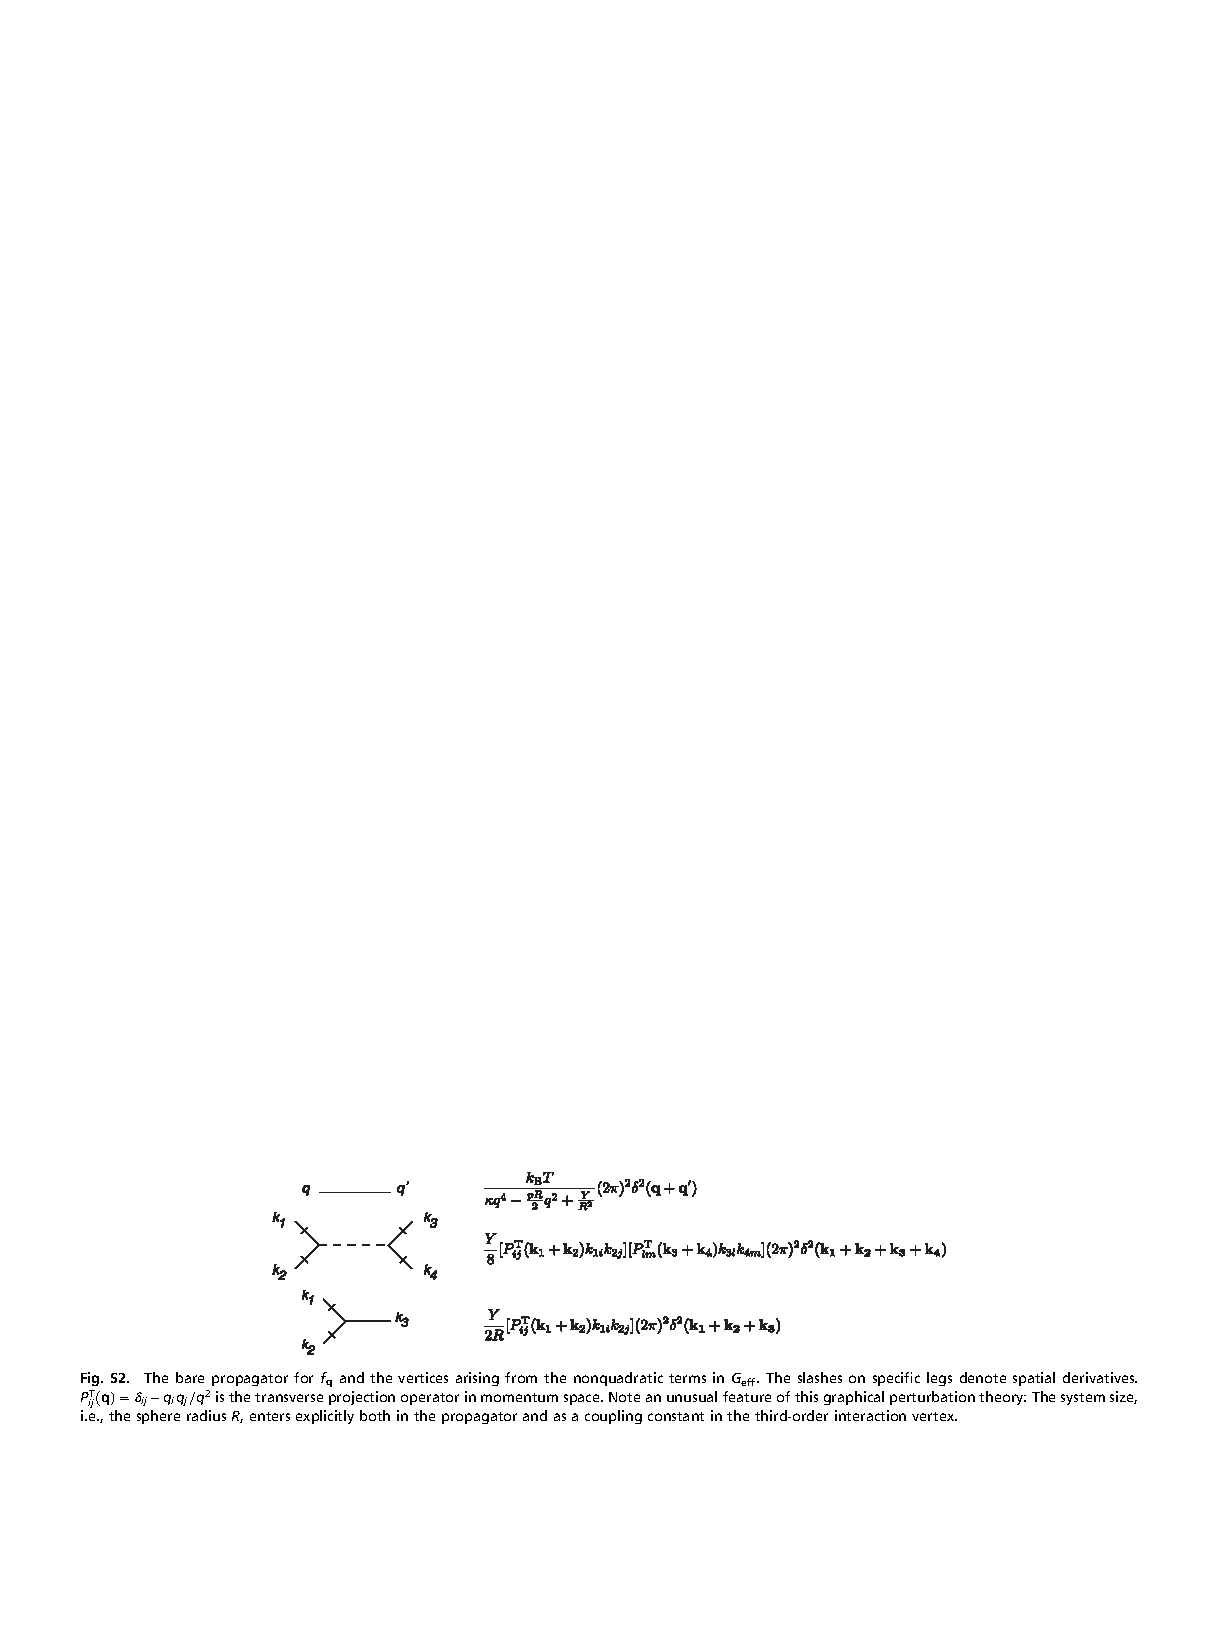
\includegraphics[width=4in]{nelsonS2}
\caption{
غشا با هندسه‌ی کروی.
}
\label{fig:nelsonS2}
\end{center}
\end{figure}

\begin{figure}[h]
\begin{center}
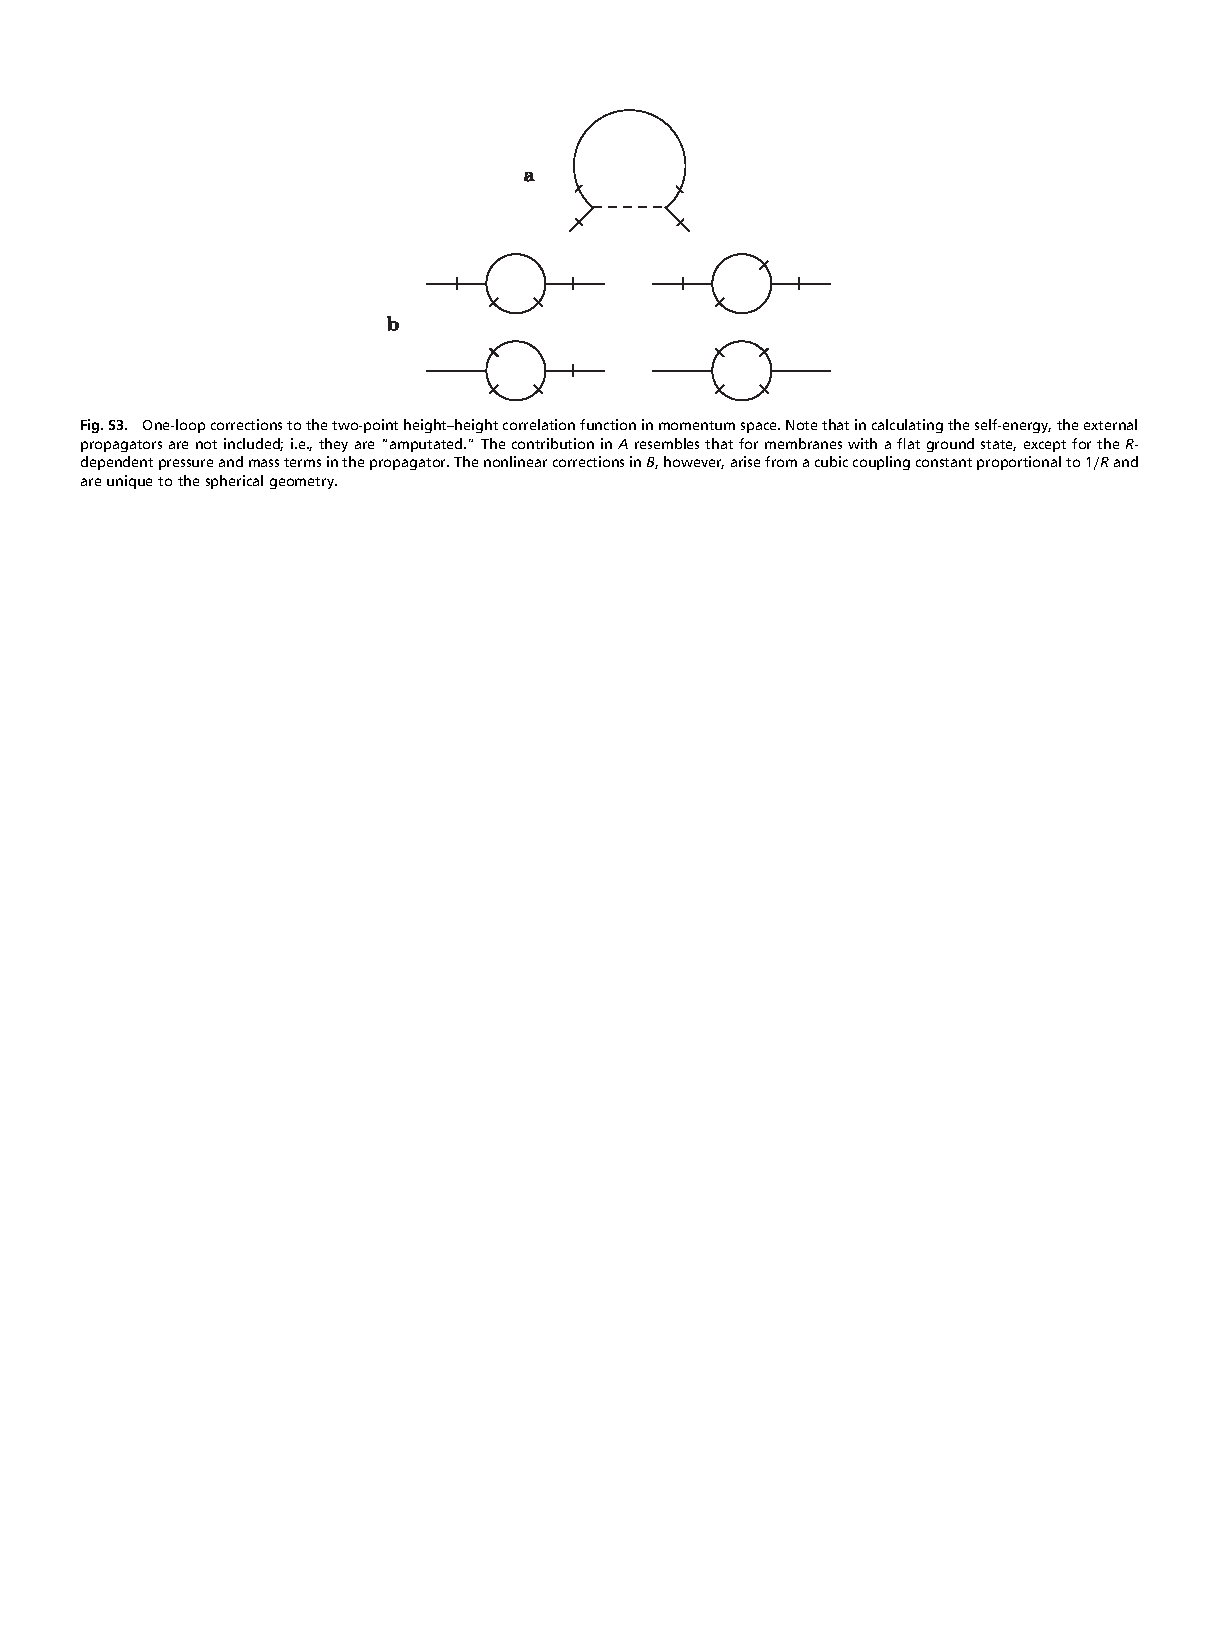
\includegraphics[width=4in]{nelsonS3}
\caption{
غشا با هندسه‌ی کروی.
}
\label{fig:nelsonS3}
\end{center}
\end{figure}
X
 قوانین فاینمن برای برگرفته شده از معادله‌ی \ref{eq:nelsonS15} 
 در شکل \ref{fig:nelsonS2}
 خلاصه شده است. از این پس مؤلفه‌های تبدیل فوریه به شکل
 $f_{\boldsymbol q}=\int d^2xf(\boldsymbol x)\exp(i\boldsymbol q.\boldsymbol x)$
 تعریف می‌شود. تبدیل فوریه‌ی وارون تغییر شکل‌های خارج از صفحه نیز به صورت
\begin{equation}
f(\boldsymbol x)=\frac{1}{A}\sum_{\boldsymbol q\neq 0}f_{\boldsymbol q}e^{-i\boldsymbol q.\boldsymbol x}
\label{eq:nelsonSٓ18}
\end{equation}
تعریف می‌شود و جمع روی تمام طول موج‌های مجاز است. خود انرژی ناشی از جمله‌ی ناهماهنگ ۳ نقطه‌ای و ۴ نقطه‌ای در شکل \ref{fig:nelsonS3}
الف خلاصه شده‌اند و این جملات برای توصیف غشای تخت نیز لازم هستند و به شکل 
\begin{equation}
-Y\int\frac{d^2k}{(2\pi)^2}\frac{\left[P_{ij}^Tq_iq_j\right]^2}{\kappa|\boldsymbol q + \boldsymbol k|^4-\frac{pR}{2}|\boldsymbol q + \boldsymbol k|^2+\frac{Y}{R^2}}
\label{eq:nelsonS19}
\end{equation}
 مجموع جملات خود انرژی ناشی از نمودارهای \ref{fig:nelsonS3}
 ب،

\begin{equation}
\begin{aligned}
\frac{Y^2}{R^2} &\int\frac{d^2k}{(2\pi)^2} \frac{1}{ 
\left( \kappa|\boldsymbol q + \boldsymbol k|^4 - \frac{pR}{2} |\boldsymbol q + \boldsymbol k|^2 + \frac{Y}{R^2} \right)
\left( \kappa k^4 - \frac{pR}{2}k^2 + \frac{Y}{R^2} \right) 
} \\
&\times\left\{ 
\frac{1}{2} \left[ P_{ij}^T(\boldsymbol q)k_ik_j\right]^2 + 
\left[P_{ij}^T(\boldsymbol k)q_iq_j\right]^2 + 
\left[P_{ij}^T(\boldsymbol k)q_iq_j\right] 
\left[P_{lm}^T(\boldsymbol{k+ q})q_lq_m\right] \right.\\
& \left.+ 2\left[P_{ij}^T(\boldsymbol k)q_iq_j\right]
\left[P_{lm}^T(\boldsymbol{q})k_lk_m\right]
\right\}
\label{eq:nelsonS20}
\end{aligned}
\end{equation}
وارون تابع همبستگی هماهنگ که در معادله‌ی \ref{eq:nelsonS17} مشاهده کردید فقط از جملات $q^0$، $q^2$، و $q^4$ تشکیل شده است و تصحیحات تک حلقه (که در معادلات \ref{eq:nelsonS19} و \ref{eq:nelsonS20} محاسبه شد) انجام شده به طیف جملاتی با همین توان‌ها و همچنین جملاتی با مرتبه‌ی $q^6$ نیز اضافه می‌کند. اگر  تصحیحات را تنها تا مرتبه‌ی $q^4$ نگه داریم می‌توانیم طیف را برای $q$های
کوچک تقریب بزنیم. 
\begin{equation}
Ak_BT\left\langle|f_{\boldsymbol q\rightarrow \boldsymbol 0}|^2\right\rangle^{-1} \equiv\kappa_Rq^4-\frac{p_RR}{2}q^2+\frac{Y_R}{R^2}+O(q^6)
\label{eq:nelsonS21}
\end{equation}
 که در بالا $Y_R$، $\kappa_R$، و $p_R$ به ترتیب مدول یانگ مؤثر، سختی خمش مؤثر، و فشار بی بعد. در مقیاس‌های طولی بزرگ اندازه‌گیری مشخصات کشسانی پوسته‌هایی که با گرما افت و خیز می‌کنند اطلاعاتی در مورد مشخصات مؤثر کشسانی در اختیار ما قرار می‌دهد. استفاده از این مشخصات بهتر از استفاده از مدول‌های خام $Y$، $\kappa$، و $p$
است که با تقریب دمای صفر رفتار پوسته در دما توصیف می‌کنند. با استفاده از معادلات \ref{eq:nelsonS19} و \ref{eq:nelsonS20} 
تا مرتبه‌ی $O(q^4)$
می‌توان انتگرال‌های تکانه را برای خود انرژی محاسبه کنیم،
\begin{equation}
Y_R=Y\left[1-\frac{3}{128\pi}\frac{k_BT}{\kappa}\frac{\sqrt\gamma}{(1-\eta^2)^{3/2}}\left(\eta\sqrt{1-\eta^2}+\pi-\cos^{-1}\eta\right)\right]
\label{eq:nelsonS22}
\end{equation}

\begin{equation}
\begin{aligned}
\kappa_R&=\kappa\left[1+\frac{1}{30720\pi}\frac{k_BT}{\kappa}\frac{\sqrt\gamma}{(1-\eta^2)^{7/2}}\right.\\
&\left.\left[\times\eta\sqrt{1-\eta^2}(-1699+3758\eta^2-2104\eta^4) \right.\right.\\
& \left.\left. +15(61-288\eta^2+416\eta^4-192\eta^6)(\pi-\cos^{-1}\eta)\right]\right]
\label{eq:nelsonS23}
\end{aligned}
\end{equation}

\begin{equation}
\begin{aligned}
\eta_R&=\eta+\frac{1}{1536\pi}\frac{k_BT}{\kappa}\frac{\sqrt\gamma}{(1-\eta^2)^{5/2}}\\
&\times\left[\sqrt{1-\eta^2}(64-67\eta^2)+3(21\eta-22\eta^3)(\pi-\cos^{-1}\eta)\right]
\label{eq:nelsonS24}
\end{aligned}
\end{equation} 
و در معادلات بالا فشار بی بعد $\eta=p/p_c$
تعریف کردیم. به طور مشخص زمانی که $\eta\rightarrow1$
این کمیت‌ها به بی‌نهایت میل می‌کنند. این جملات برای پایین‌ترین مرتبه فشار خارجی به شکل زیر تقریب زده می‌شوند،
 \begin{equation}
Y_R\approx Y\left[1-\frac{3}{256}\frac{k_BT}{\kappa}\sqrt\gamma\left(1+\frac{4}{\pi}\frac{p}{p_c}\right)\right]
\label{eq:nelsonS25}
\end{equation}

\begin{equation}
p_R\approx p+\frac{1}{24\pi}\frac{k_BT}{\kappa}p_c\sqrt\gamma\left(1+\frac{63\pi}{128}\frac{p}{p_c}\right)
\label{eq:nelsonS26}
\end{equation}

\begin{equation}
\kappa_R\approx \kappa\left[1+\frac{61}{4096}\frac{k_BT}{\kappa}\sqrt\gamma\left(1-\frac{1568}{915\pi}\frac{p}{p_c}\right)\right]
\label{eq:nelsonS27}
\end{equation}
برای محاسبه‌ی انتگرال‌های بالا باید از انتگرال‌های معادلات \ref{eq:nelsonS19} و \ref{eq:nelsonS20} روی تمام طول‌ موج‌های مجاز فضای فاز انتگرال بگیریم. طول‌ موج‌ها از حد پایین $k_{min}\sim1/R$ تا حد بالای طول موج‌ که با ثابت میکروسکوپیک شبکه‌ی شبکه تعیین می‌شود، است. از آنجایی که تمام انتگرال‌ها در حد بالا به حد فرابنفش همگرا می‌شوند می‌ توانیم $k\rightarrow\infty$. به علت وجود جمله‌ی «جرم» $\sim Y/R^2$ انتگرال در محدوده‌ی طول موج‌های کوچک خوش رفتار است، و در نتیجه می‌توان انتگرال را در این محدوده روی تمام فضای فاز دو بعدی انجام دهیم. اینکه انتگرال را برای محدوده‌ی پایین‌تر از فروسرخ یا $0<k<1/R$ انجام دهیم باعث ایجاد خطای از مرتبه‌ی $1/\sqrt\gamma$ می‌شود که برای پوسته‌های خیلی نازک قابل صرف نظر کردن است. 

با نگاه کردن به معادلات $\ref{eq:nelsonS25}، $\ref{eq:nelsonS26}، و \ref{eq:nelsonS27} می‌بینیم که در حد طول موج‌های بلند تغییر شکل‌های تابع مدول یانگ موثر کوچکتر، سختی خمش مؤثر بزرگتر، و کشش سطحی غیر صفر منفی است. این رفتار حتی وقتی که فشار خارجی صفر باشد نیز صادق است. وقتی $p/p_c$ بزرگ باشد، مدول یانگ و سختی خمش از تقریب دمای صفر کوچکتر می‌شوند و اندازه‌ی کشش سطحی مؤثر منفی که با $p_c$ تعیین می‌شود بسیار بزرگ می‌شود. محاسبات خطاهای مرتبه‌های بالاتر همگی نشان می‌دهند که با $p/p_c\rightarrow1$ تمام تصحیحات به بی‌نهایت میل می‌کنند. همچنین مشا‌هده می‌کنیم که تمام مشخصات مؤثر تابع دما و اندازه‌ی سیستم هستند زیرا که $\sqrt\gamma\sim R$ . با اینکه برای $k_BT\ll\kappa$ 
سهم تصحیحات ناچیز است ولی باید در نظر بگیریم که با بزرگ شدن شعاع سیستم $R\rightarrow\infty$ 
به بینهایت میل می‌کند. 


کشش سطحی ناشی از افت و خیز گرمایی و تابعیت قوی آن با فشار خارجی، همچنین تابعید ثابت کشسانی سیستم با اندازه‌ی سیستم مشخصات مختص غشاهای کروی است و در غشا‌های تخت دیده نمی‌شود. 
\section{بررسی با استفاده از هماهنگ‌های کروی}
یک پوسته‌ی کروی با شعاع $R$، سختی خمش $\kappa$ و مؤلفه‌های لامه $\mu$ و $\lambda$ 
در نظر بگیرید که تحت یک میدان مماسی $\boldsymbol u(u_x,u_y)$
و میدان جابجایی شعاعی $f$
قرار گرفته‌است. میدان $\boldsymbol u$
را مانند تمام میدان‌های خوش رفتار می‌توان مجموع یک بخش بدون چرخش
\LTRfootnote{curl free}
و بخش بدون واگرایی
\LTRfootnote{divergence free}
نوشت، $\boldsymbol u\equiv\nabla\boldsymbol\Psi+\boldsymbol v$ که تابع اسکالر $\boldsymbol\Psi$ قسمت غیرچرخش
\LTRfootnote{irrotational}
 را تولید می‌کند و $\boldsymbol v$ بخش مارپیچی
 \LTRfootnote{solenoidal}
 است. در بخش شعاعی مختصات شعاعی نود $i$ 
 در مختصات زاویه‌ای $(\theta,\phi)$ را می‌توانیم به شکل $r_i(\theta,\phi)=R_0+f(\theta,\phi)$
 نوشت و $R_0$ در اینجا شعاع متوسط کره‌ی در حال افت و خیز است.
 هنگام بسط دادن بر حسب هماهنگ‌ها کروی حقیقی به شکل
\begin{equation}
\begin{aligned}
&f(\theta,\phi)=R\sum_{l=0}^{l_M}\sum_{m=-l}^{m=l}A_{lm}Y_{lm}(\theta,\phi)\\
&\boldsymbol\Psi(\theta,\phi)=R^2\sum_{l=0}^{l_M}\sum_{m=-l}^{m=l}B_{lm}Y_l^m(\theta,\phi)
\label{eq:nelsonS28.1}
\end{aligned}
\end{equation} 

خواهند بود و انرژی کشسانی تغییر شکل آن تا مرتبه‌ی دوم تحت این میدان‌ها طبق معادله‌ی زیر خواهد بود \cite{krollPRE1993}

\begin{equation}
\begin{aligned}
G&=R^2\sum_{l,m}\left\{\left[\frac{\kappa}{2}\frac{(l+2)^2(l-1)^2}{R^2}+2K\right]A_{lm}^2-2Kl(l+1)A_{lm}B_lm\right.\\
&\left.+\frac{1}{2}l(l+1)[(K+\mu)l(l+1)-2\mu]B_{lm}^2\right\}+G_{sol}(\boldsymbol v)
\label{eq:nelsonS28}
\end{aligned}
\end{equation} 
که در اینجا $K=\mu+\lambda$
برابر مدول حجمی‌ 
\LTRfootnote{bulk modulus}
است. قسمت مارپیچی باعث انرژی در جابجایی شعاعی نشده و انرژی جداگانه با تابعیت $\boldsymbol v$ با تابعیت مربعی دارد. همچنین به معادله‌ی بالا انرژی ناشی از کشش سطحی منفی $-pR/2$ که در اثر انقباض ناشی از وجود فشار خارجی بوجود می‌آید را به صورت $G_s=-(pR/2)\Delta A$ اضافه می‌کنیم. در اینجا $\Delta A$ سطحی مضاعفی است که به علت تغییر شکل نسبت به شعاع میانگین ایجاد می‌شود. می‌توان میزان سطح مضاعف را بر حسب هماهنگ‌های کروی نوشت.
\cite{milnersafranPRA1987}
\begin{equation}
\Delta A\approx R^2\sum_{l>1,m}A_{lm}^2\left[1+\frac{l(l+1)}{2}\right]
\label{eq:nelsonS29}
\end{equation} 
همانند تقریب انرژی کشسانی پوسته‌های کم عمق اینجا نیز روی جملات مرتبه‌ی دوم $B_{lm}$ و $\boldsymbol v$ انتگرال می‌گیریم و انرژی آزاد مؤثر سیستم را بر حسب جابجایی شعاعی می‌نوسیم،
\begin{equation}
\begin{aligned}
&G_{eff}&=\frac{R^2}{2}\sum_{l>1,m}\left\{\frac{\kappa(l+2)^2(l-1)^2}{R^2}-pR\left[1+\frac{l(l+1)}{2}\right]\right.\\
&\left.+\frac{4\mu(\mu+\lambda)(l^2+l-2)}{(2\mu+\lambda)(l^2+l)-2\mu}\right\}A_{lm}^2
\label{eq:nelsonS30}
\end{aligned}
\end{equation} 
 با توجه به نظریه هم پاری انرژی،
\begin{equation}
\begin{aligned}
k_BT\left\langle|A_{lm}|^2\right\rangle_0^{-1}&=\\
&\kappa(l+2)^2(l-1)^2-pR^3\left[1+\frac{l(l+1)}{2}\right]+\frac{4\mu(\mu+\lambda)(l^2+l+2)}{(2\mu+\lambda)(l^2+l)-2\mu}R^2\\
&=\kappa(l+2)^2(l-1)^2-pR^3\left[1+\frac{l(l+1)}{2}\right]+\frac{Y}{1+\frac{Y}{2\mu(l^2+l-2)}}R^2
\label{eq:nelsonS31}
\end{aligned}
\end{equation} 
که $Y$ مدول یانگ ۲ بعدی است که قبل‌تر تعریف کردیم. حالا می‌توانیم با استفاده از پارامتر‌های وابسته به دمای مؤثر $Y_R$، $\kappa_R$، و $p_R$ به جای پارامتر‌های پایه‌ای تغییرات در افت خیز ناشی از گرما را تعریف کرد. ولی برای محاسبه‌ی آخرین جمله در معادله‌ی \ref{eq:nelsonS31} 
نیاز داریم تصحیحات گرمایی وارد بر مؤلفه‌های لامه $\mu$
و $\lambda$ 
را بدانیم. در محاسبات مربوط به نظریه‌ی پوسته‌های کم عمق این مؤلفه‌ها در محاسبات نهایی حذف شدند. در شبیه‌سازی که در مطالعه‌ی 
\cite{gomppernelson2012}
برای انرژی کشسانی گسسته‌سازی شده $\mu=3Y/8$
محاسبه شده. اگر فرض کنیم که تصحیحات گرمایی ناشی از مرتبه‌ی تک حلقه ناچیز است می‌توانیم فرض کنیم که $Y_R\approx Y$ 
است. با جایگذاری در معدله‌ی \ref{eq:nelsonS31} به همراه پارمتر‌های مؤثر دیگر به شکل نهایی زیر می‌رسیم،
\begin{equation}
\begin{aligned}
k_BT\left\langle|A_{lm}|^2\right\rangle^{-1}&\approx\\
&\kappa_R(l+2)^2(l-1)^2-p_RR^3\left[1+\frac{l(l+1)}{2}\right]+Y_RR^2\left[\frac{3(l^2+l-2)}{3(l^2+l)-2}\right]
\label{eq:nelsonS32}
\end{aligned}
\end{equation} 
حتی اگر تصحیحات گرمایی وارد بر $\mu$
و $Y$
از مرتبه‌ی $O(k_BT)$ 
باشد می‌توان اختلاف خطای اضافه شده هنگامی که فرض کردیم $\mu_R\approx3Y_R/8$
حد بالای 
$4[3(l^2+l-2)+4]$
نسبت به تغییرات ناهماهنگ دارد و در نتیجه هنگامی که $l>1$
یک مرتبه‌ی بزرگی کوچکتر خواهد بود.


%\renewcommand{\refname}{whatever}
%\bibliography{reference} 
%\bibliographystyle{IEEEtran}
%\renewcommand\refname{مراجع}


	        
	       